\documentclass{article}
\usepackage[utf8]{inputenc}
\usepackage{graphicx}
\usepackage{amsmath }
\usepackage{amssymb}
\usepackage{subcaption}
\usepackage{float}
\usepackage{multirow}
\usepackage{nomencl}
\usepackage{bm}
\usepackage{hyperref}
\usepackage[makeroom]{cancel}
\usepackage{algorithm}
\usepackage{algorithmic}
\setcounter{section}{1}


\usepackage{cleveref} %referencing figures, equations and tables
\crefformat{figure}{Figure.~#2#1#3}
\crefformat{equation}{Eq.~#2#1#3}
\crefformat{table}{Table.~#2#1#3}
\crefformat{appendix}{Appendix.~#2#1#3}
\crefformat{section}{Section.~#2#1#3}

\title{Lekhnitskii Formulation for Stress Concentration Around A Circular Hole in A Thin Orthotropic Plate}
\author{Amir Baharvand }
\date{}

\begin{document}

\maketitle

\makenomenclature

\nomenclature[T]{\textbf{Balanced laminate}}{A laminate in which the number of plies with $\pm\theta$ are equal.}
% \nomenclature[T]{\textbf{Angle-ply laminate}}{An angle-ply laminate includes only 0$^\text{o}$ and/or 90$^\text{o}$ plies with the same material and thickness.}
\nomenclature[T]{\textbf{Analytical function}}{A complex function is called analytical / Holomorphic over a region $R$ is it is differentiable at any point in region $R$.}
% \nomenclature[T]{\textbf{Cross-ply function}}{A cross-ply laminate includes $\pm\theta$ plies with the same material and thickness.}
\nomenclature[T]{\textbf{Fundamental theorem of Algebra}}{If two series are equal, either finite or infinite, then the coefficient of their like powers are equal.}

\nomenclature[S]{1}{Ply local coordinate (horizontal axis)}
\nomenclature[S]{2}{Ply local coordinate (vertical axis)}
\nomenclature[S]{3}{Ply local coordinate}
\nomenclature[S]{s}{sine}
\nomenclature[S]{c}{cosine}
\nomenclature[S]{t}{Total}

\nomenclature[L]{$x$}{$x$-axis}
\nomenclature[L]{$y$}{$y$-axis}
\nomenclature[L]{$z$}{$z$-axis}
\nomenclature[L]{$\bm{C}$}{Stiffness tensor}
\nomenclature[L]{$\bm{S}$}{Compliance tensor}
\nomenclature[L]{$\bm{S^{'}}$}{Transformed compliance tensor}
\nomenclature[L]{$\mathfrak{S}$}{Sign}
\nomenclature[L]{$u$}{Displacement along $x$-axis}
\nomenclature[L]{$v$}{Displacement along $y$-axis}
\nomenclature[L]{$w$}{Displacement along $z$-axis}
\nomenclature[L]{$E$}{Young's modulus}
\nomenclature[L]{$h$}{Thickness}
\nomenclature[L]{$\bm{R}$}{Reuter matrix}
\nomenclature[L]{$\bm{M}$}{Transformation matrix}
\nomenclature[L]{$\bm{Q}$}{Orthogonal tensor/Reduced stiffness matrix}
\nomenclature[L]{$h_k$}{Homogeneous Stress Field}
\nomenclature[L]{$A_k$}{Force Resultant Around Hole}
\nomenclature[L]{$g_n^{(k)}$}{Disturbance Field}
\nomenclature[L]{$U$}{Body force}
\nomenclature[L]{$\overline{u}$}{Average displacement along $x$-axis}
\nomenclature[L]{$\overline{v}$}{Average displacement along $y$-axis}
\nomenclature[L]{$\overline{U}$}{Average body force}
\nomenclature[L]{$V$}{Potential function}
\nomenclature[L]{$\overline{X}$}{Average prescribed traction along $x$-axis}
\nomenclature[L]{$\overline{Y}$}{Average prescribed traction along $y$-axis}
\nomenclature[L]{$\overline{u}^*$}{Average prescribed displacement along $x$-axis}
\nomenclature[L]{$\overline{v}^*$}{Average prescribed displacement along $y$-axis}
\nomenclature[L]{$n$}{Normal vector}
\nomenclature[L]{$s$}{Complex variable/Characteristic equation roots/infinitesimal element}
\nomenclature[L]{$f$}{Potential stress function solution}
\nomenclature[L]{$\mathfrak{Re}$}{Real}
\nomenclature[L]{$\mathfrak{Im}$}{Imaginary}
\nomenclature[L]{$u_0$}{Rigid body displacement along $x$-axis}
\nomenclature[L]{$v_0$}{Rigid body displacement along $y$-axis}
\nomenclature[L]{$X$}{Prescribed traction along $x$-axis}
\nomenclature[L]{$Y$}{Prescribed traction along $y$-axis}
\nomenclature[L]{$\bm{A}$}{A matrix in ABD matrix}
\nomenclature[L]{$\bm{B}$}{B matrix in ABD matrix}
\nomenclature[L]{$\bm{D}$}{D matrix in ABD matrix}
\nomenclature[L]{$\bm{a}$}{a matrix in ABD inverse matrix}
\nomenclature[L]{$\bm{b}$}{b matrix in ABD inverse matrix}
\nomenclature[L]{$\bm{c}$}{c matrix in ABD inverse matrix}
\nomenclature[L]{$\bm{d}$}{d matrix in ABD inverse matrix}
\nomenclature[L]{$p$}{Prescribed stress}
\nomenclature[L]{$N$}{Normal resultant load}
\nomenclature[L]{$T$}{Tangential resultant load}
\nomenclature[L]{$r$}{Radius}
\nomenclature[L]{$R$}{Resultant load}

\nomenclature[G]{$\sigma$}{Normal stress}
\nomenclature[G]{$\epsilon$}{Normal strain}
\nomenclature[G]{$\omega_0$}{Rigid body rotation}
\nomenclature[G]{$\mu$}{Shear modulus}
\nomenclature[G]{$\nu$}{Poisson's ratio}
\nomenclature[G]{$\tau$}{Shear stress}
\nomenclature[G]{$\overline{\sigma}$}{Average normal stress}
\nomenclature[G]{$\overline{\tau}$}{Average shear stress}
\nomenclature[G]{$\gamma$}{Shear strain}
\nomenclature[G]{$\overline{\gamma}$}{Average shear strain}
\nomenclature[G]{$\theta$}{Angle}
\nomenclature[G]{$\phi$}{Potential stress function}
\nomenclature[G]{$\Theta$}{Angle of hole}
\nomenclature[G]{$\alpha$}{Real part of complex solution}
\nomenclature[G]{$\beta$}{Imaginary part of complex solution}

\printnomenclature
\tableofcontents

\section*{Abstract}
Lekhnitskii formalism is one of the few approaches in analyzing anisotropic elastic bodies which essentially is the generalization of Muskhelishvili formalism for isotropic elastic bodies. Lekhnitskii theory starts by deriving stresses from the equilibrium equation, then follows the compatibility to solve strains and finally calculate displacement fields. In this methodology, a potential function approach, analogous to the Airy stress function, along with complex analysis is invoked. The goal of the present report is to derive the generalized Lekhnitskii theory and then apply it to a thin orthotropic laminate containing a hole.

\section{Introduction}
Lekhnitskii theory for anisotropic elastic bodies is a robust tool in analyzing the stretching, bending and stretch-bending coupling of composite laminates. This theory provides an analytical approach to analyze the stress and displacement field in composite laminates with/without cut-off (also known as irregularity as used in \cite{Koussios2009}) which are very common in the aerospace industry, \emph{e.g}, riveted holes and elliptical or rounded rectangular windows in civilian aircraft.\\

The present report is divided into three main sections. In the first, we discuss the general theory of Lekhnitskii. The second section narrows the Lekhnitskii theory to thin orthotropic laminates and in the last section, we invoke the Classical Composite Laminate Theory along with the Lekhnitskii theory to find the stress field around an infinite plate with a circular hole under biaxial loading. \\

Despite the derivation of all equations, in subsequent sections, most of the contents are borrowed from \cite{Lekhnitskii1968} and \cite{Jong1987}.
\section{Plane Problem in Linear Elasticity of An Anisotropic Body }

\subsection{Generalized Plane Stress Theory}
The generalized plane stress was introduced to overcome the peculiar dependency of the displacements on $z$ in the plane stress. The whole idea of the generalized plane stress is upon averaging the stress and displacement over the domain thickness to remove the $z$ dependency. The generalized plane stress assumes

\begin{enumerate}
    \item The domain is bounded between two parallel planes, here $z=\pm h$ (see \cref{fig:gen_plane_stress}) where both planes are either traction-free or symmetrically loaded through the thickness so that their average value over the thickness vanishes.
    \item The plate thickness is negligible w.r.t. the other geometrical dimension.
    \item Body forces are independent of $z$ or symmetrically distributed through the thickness.
    \item The displacement along the $z$-axis is an odd function that is $w(x, y, z) = -w(x, y, -z)$, in other words, the mid-plane does not undergo bending.
    \item Deformations are infinitesimal.
\end{enumerate}

\begin{figure}[H]
    \centering
    \includegraphics[width = 0.55\textwidth ]{figures/gen_plane_stress.pdf}
    \caption{The elastic body representing the generalized plane stress. The shaded area represents the mid-plane.}
    \label{fig:gen_plane_stress}
\end{figure}

\cref{fig:gen_plane_stress} illustrates the generalized plane stress. The origin is placed at the mid-plane center and $h$ indicates the plate thickness. As mentioned earlier, the values of stress and displacement are averaged over the plate thickness in this theory; therefore,

\begin{equation}
    \begin{matrix}
    \overline{\sigma}_x = \dfrac{1}{2h} \displaystyle\int_{-h}^{h} \sigma_x \mathrm{d}z & , 
    \overline{\sigma}_y = \dfrac{1}{2h} \displaystyle\int_{-h}^{h} \sigma_y \mathrm{d}z & , 
    \overline{\tau}_{xy} = \dfrac{1}{2h} \displaystyle\int_{-h}^{h} \tau_{xy} \mathrm{d}z \\
    \\
    \overline{\sigma}_z = \dfrac{1}{2h} \displaystyle\int_{-h}^{h} \sigma_z \mathrm{d}z & ,
    \overline{u} = \dfrac{1}{2h} \displaystyle\int_{-h}^{h} u \mathrm{d}z & ,
    \overline{v} = \dfrac{1}{2h} \displaystyle\int_{-h}^{h} v \mathrm{d}z
    \end{matrix}
\end{equation}

$\sigma$ and $\tau$ designate the normal and shear stress, $u$ and $v$ are the displacements in the $x$ and $y$-direction, respectively. The rest of variables with a bar sign indicate the corresponding average value. The subscripts also indicate the coordinate axis. While $\sigma_z$ is negligible compared to other stress components, it is worth noting that the value of $\overline{\sigma}_z$ is zero as it is assumed to be symmetric w.r.t the mid-plane. \\

\subsection{Field Equations}
The equilibrium equation for the generalized plane stress reduces to 

\begin{gather}
    \frac{\partial \overline{\sigma}_x}{\partial x} + \frac{\partial \overline{\tau}_{xy}}{\partial y} + \overline{U}_x = 0 \notag\\
    \frac{\partial \overline{\tau}_{xy}}{\partial x} + \frac{\partial \overline{\sigma}_y}{\partial y} + \overline{U}_y = 0 
    \label{eq:equilibrium_eqn}
\end{gather}

where $\overline{U_x}$ and $\overline{U_y}$ are average body force per unit volume along $x$ and $y$ axes and are 

\begin{equation}
    \begin{matrix}
    \overline{U}_x = \dfrac{1}{2h} \displaystyle\int_{-h}^{h} U_x \mathrm{d}z & , 
    \overline{U}_y = \dfrac{1}{2h} \displaystyle\int_{-h}^{h} U_y \mathrm{d}z
    \end{matrix}
\end{equation}

For a composite laminate with fibers oriented in angles other than 0 and/or 90 degrees, some nonzero coupling terms appear in the compliance tensor, $\bm{S^{'}}$. For such laminate the stress-strain ($\bm{\sigma}-\bm{\epsilon}$) relation is \cite{Kassapoglou2015}

\begin{equation}
\begin{Bmatrix}
\overline{\epsilon}_x\\ 
\overline{\epsilon}_y\\ 
\overline{\epsilon}_z\\
\overline{\gamma}_{yz}\\ 
\overline{\gamma}_{zx}\\
\overline{\gamma}_{xy}\\
\end{Bmatrix}
=\begin{bmatrix}
S^{'}_{11} & S^{'}_{12} & S^{'}_{13} & 0 & 0 & S^{'}_{16} \\ 
S^{'}_{12} & S^{'}_{22} & S^{'}_{23} & 0 & 0 & S^{'}_{26} \\ 
S^{'}_{13} & S^{'}_{23} & S^{'}_{33} & 0 & 0 & S^{'}_{36} \\ 
0 & 0 & 0 & S^{'}_{44} & S^{'}_{45} & 0 \\ 
0 & 0 & 0 & S^{'}_{45} & S^{'}_{55} & 0 \\ 
S^{'}_{16} & S^{'}_{26} & S^{'}_{36} & 0 & 0 & S^{'}_{66}
\end{bmatrix}
\begin{Bmatrix}
\overline{\sigma}_x\\ 
\overline{\sigma}_y\\ 
0\\ 
0\\ 
0\\
\overline{\tau}_{xy}
\end{Bmatrix}
\label{eq:stress_strain}
\end{equation}

The components of the compliance tensor are given in \cref{app:compliance_mat}. For the generalized stress sate, \cref{eq:stress_strain} reduces to 

\begin{gather}
    \overline{\epsilon}_x = S^{'}_{11} \overline{\sigma}_x + S^{'}_{12} \overline{\sigma}_y + S^{'}_{16} \overline{\tau}_{xy} \notag\\
    \overline{\epsilon}_y = S^{'}_{12} \overline{\sigma}_x + S^{'}_{22} \overline{\sigma}_y + S^{'}_{26} \overline{\tau}_{xy} \notag\\
    \overline{\gamma}_{xy} = 2\overline{\epsilon}_{xy} = S^{'}_{16} \overline{\sigma}_x + S^{'}_{26} \overline{\sigma}_y + S^{'}_{66} \overline{\tau}_{xy}
    \label{eq:average_stress_strain}
\end{gather}

The strain-displacement can be written as

\begin{equation}
    \overline{\epsilon}_{\alpha\beta} = \frac{1}{2}(\overline{u}_{\alpha, \beta} + \overline{u}_{\beta, \alpha})
    \label{eq:strain}
\end{equation}

where $\alpha$ and $\beta$ occupy $x$ and $y$, $\overline{\epsilon}$ and $\overline{\gamma}$ are the average normal and shear strain over the thickness. The compatibility equation can be calculated by properly differentiating the displacement components in \cref{eq:strain} (see \cref{app:compatibility_eqn} for the derivation).

\begin{equation}
    \dfrac{\partial^2 \overline{\epsilon}_x}{\partial y^2} + \dfrac{\partial^2 \overline{\epsilon}_y}{\partial x^2} - \dfrac{\partial^2 \overline{\gamma}_{xy}}{\partial x \partial y} = 0
    \label{eq:compatibility}
\end{equation}

Assuming that the body forces can be derived from a potential function, $V$ such that

\begin{equation*}
    \begin{matrix}
    \overline{U}_x = -\dfrac{\partial \overline{V}}{\partial x} & , 
    \overline{U}_y = -\dfrac{\partial \overline{V}}{\partial y}
    \end{matrix}
\end{equation*}

the stress components (see \cref{eq:equilibrium_eqn}) can be expressed via the following set of equations.

\begin{equation}
    \begin{matrix}
    \overline{\sigma}_x = \dfrac{\partial^2 \phi}{\partial y^2} + \overline{V} & , 
    \overline{\sigma}_y = \dfrac{\partial^2 \phi}{\partial x^2} + \overline{V} & , 
    \overline{\tau}_{xy} = -\dfrac{\partial^2 \phi}{\partial x \partial y}
    \end{matrix}
    \label{eq:average_stress}
\end{equation}

where $\phi = \phi(x, y)$ is called the potential stress function. Now, by replacing stress components from \cref{eq:average_stress} in \cref{eq:average_stress_strain}, the following partial differential equation is formed which should be fulfilled by the potential stress function.

\begin{multline}
    S^{'}_{22} \frac{\partial^4 \phi}{\partial x^4} - 2 S^{'}_{26} \frac{\partial^4 \phi}{\partial x^3 \partial y} + (2 S^{'}_{12} + S^{'}_{66}) \frac{\partial^4 \phi}{\partial x^2 \partial y^2} - 2 S^{'}_{16} \frac{\partial^4 \phi}{\partial x \partial y^3} + S^{'}_{11} \frac{\partial^4 \phi}{\partial y^4} \\ + (S^{'}_{12} + S^{'}_{22}) \frac{\partial^2 \overline{V}}{\partial x^2} - (S^{'}_{16} + S^{'}_{26}) \frac{\partial^2 \overline{V}}{\partial x \partial y}  + (S^{'}_{11} + S^{'}_{12}) \frac{\partial^2 \overline{V}}{\partial y^2} = 0
    \label{eq:pde_body_included}
\end{multline}

which in the absence of body forces reduces to

\begin{equation}
    S^{'}_{22} \frac{\partial^4 \phi}{\partial x^4} - 2 S^{'}_{26} \frac{\partial^4 \phi}{\partial x^3 \partial y} + (2 S^{'}_{12} + S^{'}_{66}) \frac{\partial^4 \phi}{\partial x^2 \partial y^2} - 2 S^{'}_{16} \frac{\partial^4 \phi}{\partial x \partial y^3} + S^{'}_{11} \frac{\partial^4 \phi}{\partial y^4} = 0
    \label{eq:pde_body_excluded}
\end{equation}

See \texttt{pde$\_$plane$\_$stress.mw} for the corresponding Maple file. It can be shown that a similar equation is derived in case of plane deformation (plane strain). This is proved in \cref{app:plane_strain}. \\

In general, the applied boundary conditions on an elastic body lie within three categories: (1) Traction boundary-value problems, (2) Displacement boundary-value problems and (3) Mixed traction boundary-value problems.  \\

\textbf{Traction boundary-value problems:} When an elastic body undergoes the external and body forces, then the boundary conditions can be found from

\begin{equation}
    \begin{bmatrix}
    \overline{\sigma}_x & \overline{\tau}_{xy}\\ 
    \overline{\tau}_{xy} & \overline{\sigma}_y
    \end{bmatrix} 
    \begin{Bmatrix}
    \cos(n, x) \\ 
    \cos(n, y)
    \end{Bmatrix} = 
    \begin{Bmatrix}
    \overline{\sigma}_x \cos(n, x) + \overline{\tau}_{xy} \cos(n, y) \\ 
    \overline{\tau}_{xy} \cos(n, x) + \overline{\sigma}_y \cos(n, y)
    \end{Bmatrix} = 
    \begin{Bmatrix}
    \overline{X} \\ 
    \overline{Y}
    \end{Bmatrix}
    \label{eq:average_traction}
\end{equation}

$n$ is the surface normal vector, cosine indicates the angle between the normal vector and the $x$ and $y$ axes. $\overline{X}$ and $\overline{Y}$ are the external forces in the $x$ and $y$-direction, respectively. \\

\textbf{Displacement boundary-value problems:} When the applied displacements on the surface and body forces are given.

\begin{equation}
    \begin{matrix}
    \overline{u} = \overline{u}^* & , 
    \overline{v} = \overline{v}^*
    \end{matrix}
    \label{eq:average_prescribed_displ}
\end{equation}

$\overline{u}^*$ and $\overline{v}^*$ designate the prescribed displacements on the body in $x$ and $y$-direction. \\

\textbf{Mixed traction boundary-value problems:} When both external forces and displacements are applied on portions of the surface. This case is not provided in the present report.

\subsection{Solve the Compatibility Equation in Terms of Potential Stress Function} \label{sec:solve_pde}
In the following, we remove the bar sign from the averaged values of displacement, strain and stress as well as the prime sign in the compliance tensor and neglect the body forces. \cref{eq:pde_body_excluded} changes to

\begin{equation}
    S_{22} \frac{\partial^4 \phi}{\partial x^4} - 2 S_{26} \frac{\partial^4 \phi}{\partial x^3 \partial y} + (2 S_{12} + S_{66}) \frac{\partial^4 \phi}{\partial x^2 \partial y^2} - 2 S_{16} \frac{\partial^4 \phi}{\partial x \partial y^3} + S_{11} \frac{\partial^4 \phi}{\partial y^4} = 0
    \label{eq:pde_body_excluded_rewrite}
\end{equation}

\subsubsection{Step 1: Remove \texorpdfstring{$S_{16}$}{} and \texorpdfstring{$S_{26}$}{}}
For a composite laminate with fibers oriented in angles $\pm\theta$ under tensile stress, the laminate experiences shear deformation. By transforming the fibers to the principal directions such that the original coordinate system coincides with the ply coordinate system, one is able to nullify $S_{16}$ and $S_{26}$ \cite{Kassapoglou2015}. This is demonstrated in \cref{fig:nullify}. \\

Consequently, \cref{eq:pde_body_excluded_rewrite} reduces to

\begin{equation}
    S_{22} \frac{\partial^4 \phi}{\partial x^4} + (2 S_{12} + S_{66}) \frac{\partial^4 \phi}{\partial x^2 \partial y^2} + S_{11} \frac{\partial^4 \phi}{\partial y^4} = 0
    \label{eq:pde_to_solve}
\end{equation}

$S_{11}$, $S_{12}$, $S_{22}$ and $S_{66}$ are given in \cref{eq:ortho_compliance}.

\begin{figure}[H]
    \centering
    \includegraphics[width = 0.8\textwidth ]{figures/nullify.pdf}
    \caption{$S_{16}$ and $S_{26}$ in \cref{eq:pde_body_excluded_rewrite} can be nullified by matching the original ($x-y$) and ply coordinate system (1-2) \cite{Koussios2015}}
    \label{fig:nullify}
\end{figure}

\subsubsection{Step 2: Find the Possible Solutions}
Let us assume $\phi(x, y) = f(z)$ where $z = x + sy$ is complex. See \cref{app:why_z_is_complex} for the reason of selecting $z$ as a complex expression. Using the chain role

\begin{gather*}
    \frac{\partial \phi}{\partial x} = \frac{\mathrm{d} f(z)}{\mathrm{d} z} \frac{\mathrm{d} z}{\mathrm{d} x} \xrightarrow{} \frac{\partial^4 \phi}{\partial x^4} = \frac{\mathrm{d}^4 f(z)}{\mathrm{d} z^4} \\
    \frac{\partial \phi}{\partial y} = \frac{\mathrm{d} f(z)}{\mathrm{d} z} \frac{\mathrm{d} z}{\mathrm{d} y} \xrightarrow{} \frac{\partial^4 \phi}{\partial x^4} = s^4 \frac{\mathrm{d}^4 f(z)}{\mathrm{d} z^4} \\
    \frac{\partial^2 \phi}{\partial x^2 \partial y^2} = s^2 \frac{\mathrm{d}^4 f(z)}{\mathrm{d} z^4}
\end{gather*}

\cref{eq:pde_to_solve} can be rewritten as 

\begin{gather}
    S_{22} \frac{\mathrm{d}^4 f(z)}{\mathrm{d} z^4} + (2 S_{12} + S_{66}) s^2 \frac{\mathrm{d}^4 f(z)}{\mathrm{d} z^4} + S_{11} s^4 \frac{\mathrm{d}^4 f(z)}{\mathrm{d} z^4} = 0 \notag\\
    \xrightarrow[]{\times \dfrac{1}{S_{11}}} \dfrac{S_{22}}{S_{11}} \frac{\mathrm{d}^4 f(z)}{\mathrm{d} z^4} + \dfrac{(2 S_{12} + S_{66})}{S_{11}} s^2 \frac{\mathrm{d}^4 f(z)}{\mathrm{d} z^4} + s^4 \frac{\mathrm{d}^4 f(z)}{\mathrm{d} z^4} = 0 \notag\\
    r^2 \frac{\mathrm{d}^4 f(z)}{\mathrm{d} z^4} + 2a s^2\frac{\mathrm{d}^4 f(z)}{\mathrm{d} z^4} + s^4 \frac{\mathrm{d}^4 f(z)}{\mathrm{d} z^4} = 0 \notag\\
    (r^2 + 2a s^2 + s^4) \frac{\mathrm{d}^4 f(z)}{\mathrm{d} z^4} = 0
\end{gather}

in which 

\begin{equation}
    \begin{matrix}
    r^2 = \dfrac{S_{22}}{S_{11}} & , 
    2a = \dfrac{(2 S_{12} + S_{66})}{S_{11}}
    \end{matrix}
    \label{eq:r_a}
\end{equation}

Seeking for the non-trivial solution, $\dfrac{\mathrm{d}^4 f(z)}{\mathrm{d} z^4} \neq 0$; thus,

\begin{equation}
    r^2 + 2a s^2 + s^4 = 0
    \label{eq:char_eqn}
\end{equation}

\cref{eq:char_eqn} is called the characteristic equation. It is shown by Lekhnitskii \cite{Lekhnitskiy1937} and Koussios \cite{Koussios2015} that the roots of \cref{eq:char_eqn} for an ideal elastic body (conventional material in industry) with finite and not equal to zero values of $S_{11}$, $2S_{12}+S_{66}$ and $S_{22}$ are either complex or pure imaginary. For the proof see \cref{app:complex_imag_roots}.

\subsubsection{Step 3: The Solution to the Characteristic Equation}
Let assume $s = A^2$. As a result, \cref{eq:char_eqn} becomes

\begin{equation*}
    r^2 + 2a A + A^2 = 0
\end{equation*}

which is a quadratic equation and can be easily solved.

\begin{equation*}
    A = \dfrac{-2a \pm \sqrt{4a^2 - 4r^2}}{2} = -a \pm i \sqrt{r^2 - a^2}
\end{equation*}

Next, 

\begin{align*}
    A &= -a \pm i \sqrt{r^2 - a^2} = -a \pm i \sqrt{r - a} \sqrt{r + a} &\notag \\
    & =\left(\dfrac{r-a}{2}\right) \pm 2i \sqrt{\dfrac{r-a}{2}} \sqrt{\dfrac{r+a}{2}} - \left(\dfrac{r+a}{2}\right) = \left(\sqrt{\dfrac{r-a}{2}} \pm i \sqrt{\dfrac{r+a}{2}} \right)^2 &
\end{align*}

Thus,

\begin{equation}
    s = \pm \left(\sqrt{\dfrac{r-a}{2}} \pm i \sqrt{\dfrac{r+a}{2}} \right)
    \label{eq:s_sol}
\end{equation}

\cref{eq:s_sol} can also be written as

\begin{gather}
    s_1 = \sqrt{\dfrac{r-a}{2}} + i \sqrt{\dfrac{r+a}{2}} \notag\\
    s_2 = -\sqrt{\dfrac{r-a}{2}} + i \sqrt{\dfrac{r+a}{2}} \notag\\
    s_3 = \sqrt{\dfrac{r-a}{2}} - i \sqrt{\dfrac{r+a}{2}} \notag\\
    s_4 = -\sqrt{\dfrac{r-a}{2}} - i \sqrt{\dfrac{r+a}{2}}
    \label{eq:s1_s4}
\end{gather}

Therefore, the general solution to \cref{eq:pde_to_solve} can be written as the summation of $f(z_k)$.

\begin{equation}
    \phi(x, y) = f_1(z_1) + f_2(z_2) + f_3(z_3) + f_4(z_4)
    \label{eq:phi_in_form_f}
\end{equation}

in which $z_k = x + s_k y $ where $k = 1, 2, 3, 4$. The above solution to the potential stress function implies that $f_k(z_k)$ is complex because $s_k$ is complex which indeed leads to the fact that every $f_k(z_k)$ function which is analytical does satisfy \cref{eq:phi_in_form_f}.

\subsubsection{Step 4: The Homogeneous Solution}
As mentioned earlier, the roots to the characteristic equation (\cref{eq:char_eqn}) are either complex or imaginary. Furthermore, it is also shown in \cref{app:complex_imag_roots} that $r+a$ in the set of solutions in \cref{eq:s1_s4} is positive (see \cref{app:complex_imag_roots}). Hence, we are left with two cases for $r-a$ expression.

\subsubsection*{Case 1: \texorpdfstring{$r - a \geq 0$}{}}
In this case, according to \cref{eq:s1_s4_complex}, 

\begin{equation*}
    \begin{matrix}
    s_3 = \overline{s_1} & , 
    s_4 = \overline{s_2}
    \end{matrix}
\end{equation*}

where the bar sign indicates the complex conjugate.

\subsubsection*{Case 2: \texorpdfstring{$r - a < 0$}{}}
In this case, according to \cref{eq:s1_s4_imaginary}, 

\begin{equation*}
    \begin{matrix}
    s_3 = \overline{s_2} & , 
    s_4 = \overline{s_1}
    \end{matrix}
\end{equation*}

Consequently, \cref{eq:phi_in_form_f} can be written as 

\begin{equation}
    \phi(x, y) = f_1(z_1) + f_2(z_2) + f_3(\overline{z_1}) + f_4(\overline{z_2})
    \label{eq:phi_1}
\end{equation}

for case 1 or 

\begin{equation}
    \phi(x, y) = f_1(z_1) + f_2(z_2) + f_3(\overline{z_2}) + f_4(\overline{z_1})
    \label{eq:phi_2}
\end{equation}

for case 2. Both \cref{eq:phi_1} and \cref{eq:phi_2} imply that $\phi(x,y)$ must always be real due to the existence of two complex conjugates. The general solution can be written in the form of \cref{eq:final_sol}. It is noteworthy to mention that choosing either pair (case 1 and case 2) does not affect the final solution as the imaginary parts cancel out each other \cite{Koussios2015}.

\begin{equation}
    \phi(x, y) = f_1(z_1) + f_2(z_2) + \overline{f_1(z_1)} + \overline{f_2(z_2)} = 2 \mathfrak{Re}[f_1(z_1) + f_2(z_2)]
    \label{eq:final_sol}
\end{equation}

$\mathfrak{Re}$ indicates the real part of the expression. 

\subsubsection{Summary}\label{sec:summary}
The next few lines summarize all the required information for the selection of the potential stress function to solve \cref{eq:pde_to_solve}.

\begin{enumerate}
    \item $\phi(x, y)$ should satisfy the equilibrium equation (\cref{eq:equilibrium_eqn}).
    \item $\phi(x, y)$ should satisfy the compatibility equation (\cref{eq:equilibrium_eqn}).
    \item $\phi(x, y)$ is an analytical function.
    \item $\phi(x, y)$ is real.
    \item $\phi(x, y)$ can be found from \cref{eq:final_sol} where $z_1 = x + s_1 y$ and $z_2 = x + s_2 y$ and $s_1$ and $s_2$ can be derived from \cref{eq:s1_s4}. 
    \item $\phi(x, y)$ should also satisfy the boundary condition (\cref{eq:average_traction} and \cref{eq:average_prescribed_displ}) We will further discuss this topic in \cref{sec:bvp}.
\end{enumerate}

The above list is also applicable to $f_1(z_1)$ and $f_2(z_2)$ as they both can be chosen interchangeably instead of $\phi(x, y)$.

\subsection{Stress, Strain and Displacement}
Stresses can be calculated from \cref{eq:average_stress} and \cref{eq:final_sol}.

\begin{align*}
    \sigma_x & = \dfrac{\partial^2 \phi}{\partial y^2} = \dfrac{\partial}{\partial y} \left\{ \dfrac{\partial f_1(z_1)}{\partial y} + \dfrac{\partial f_2(z_2)}{\partial y} + \dfrac{\partial \overline{f_1(z_1)}}{\partial y} + \dfrac{\partial \overline{f_2(z_2)}}{\partial y} \right\} & \\
    & = \dfrac{\partial}{\partial y} \left\{ \dfrac{\mathrm{d} f_1(z_1)}{\mathrm{d} z_1}\dfrac{\partial z_1}{\partial y} + 
    \dfrac{\mathrm{d} f_2(z_2)}{\mathrm{d} z_2}\dfrac{\partial z_2}{\partial y} +
    \dfrac{\mathrm{d} \overline{f_1(z_1)}}{\mathrm{d} z_1}\dfrac{\partial \overline{z_1}}{\partial y} +
    \dfrac{\mathrm{d} \overline{f_2(z_2)}}{\mathrm{d} z_2}\dfrac{\partial \overline{z_2}}{\partial y}
    \right\} \xrightarrow[]{\dfrac{\partial z_k}{\partial y} = s_k}  &
\end{align*}


\begin{align*}
    & = \dfrac{\partial}{\partial y} \left\{ s_1 \dfrac{\mathrm{d} f_1(z_1)}{\mathrm{d} z_1} + 
    s_2 \dfrac{\mathrm{d} f_2(z_2)}{\mathrm{d} z_2} +
    \overline{s_1} \dfrac{\mathrm{d} \overline{f_1(z_1)}}{\mathrm{d} z_1} +
    \overline{s_2}\dfrac{\mathrm{d} \overline{f_2(z_2)}}{\mathrm{d} z_2}
    \right\} & \\
    & = \dfrac{\partial}{\partial y} \left\{ s_1 \Phi_1(z_1) + s_2 \Phi_2(z_2) + \overline{s_1} \overline{\Phi_1(z_1)} + \overline{s_2} \overline{\Phi_2(s_2)} \right\} &
\end{align*}

In above equation, $\dfrac{\mathrm{d} f_k(z_k)}{\mathrm{d} z_k} = \Phi_k(z_k)$ and $\dfrac{\mathrm{d} \overline{f_k(z_k)}}{\mathrm{d} z_k} = \overline{\Phi_k(z_k)}$ where $k = 1, 2$. 

\begin{equation*}
    \dfrac{\partial}{\partial y} (s_1 \Phi_1(z_1)) = \cancelto{0}{\dfrac{\partial s_1}{\partial y}} \Phi_1(z_1) + s_1 \dfrac{\partial \Phi_1(z_1)}{\partial y} = s_1 \dfrac{\mathrm{d} \Phi_1(z_1)}{\mathrm{d} z_1} \dfrac{\partial z_1}{\partial y} = s_1^2 \dfrac{\mathrm{d} \Phi_1(z_1)}{\mathrm{d} z_1} = s_1^2 \Phi'_1(z_1) 
\end{equation*}

Repeating the above procedure for all the terms gives

\begin{equation*}
    \sigma_x = s_1^2 \Phi'_1(z_1) + s_2^2 \Phi'_2(z_2) + \overline{s_1}^2 \overline{\Phi'_1(z_1)} + \overline{s_2}^2 \overline{\Phi'_2(z_2)} = 2 \mathfrak{Re}[s_1^2 \Phi'_1(z_1) + s_2^2 \Phi'_2(z_2)]
\end{equation*}

The stress components become

\begin{gather}
    \sigma_x = 2 \mathfrak{Re}[s_1^2 \Phi'_1(z_1) + s_2^2 \Phi'_2(z_2)]  \notag \\
    \sigma_y = 2 \mathfrak{Re}[\Phi'_1(z_1) + \Phi'_2(z_2)]  \notag \\
    \tau_{xy} = -2 \mathfrak{Re}[s_1 \Phi'_1(z_1) + s_2 \Phi'_2(z_2)] 
    \label{eq:stresses}
\end{gather}

Strain can be found from \cref{eq:average_stress_strain}. For instance, 

\begin{equation*}
    \epsilon_x = S_{11} \sigma_x + S_{12} \sigma_y = 2 S_{11} \mathfrak{Re}[s_1^2 \Phi'_1(z_1) + s_2^2 \Phi'_2(z_2)] + 2 S_{12} \mathfrak{Re}[\Phi'_1(z_1) + \Phi'_2(z_2)]
\end{equation*}

The strains become

\begin{gather}
    \epsilon_x = 2 \mathfrak{Re}[(S_{11} s_1^2 + S_{12}) \Phi'_1(z_1)] + 2 \mathfrak{Re}[(S_{11} s_2^2 + S_{12}) \Phi'_2(z_2)]  \notag \\
    \epsilon_y = 2 \mathfrak{Re}[(S_{12} s_1^2 + S_{22}) \Phi'_1(z_1)] + 2 \mathfrak{Re}[(S_{12} s_2^2 + S_{22}) \Phi'_2(z_2)]  \notag \\
    \gamma_{xy} = -2 S_{66} \mathfrak{Re}[s_1 \Phi'_1(z_1) + s_2 \Phi'_2(z_2)]
    \label{eq:strains}
\end{gather}

The displacement components can be easily found by integrating the strains. The displacement along the $x$-axis, $u$, can be found by integrating $\epsilon_x$ over the $x$ axis.

\begin{align*}
    u & = \int{\epsilon_x} \mathrm{d} x + p(y) & \\
      & = 2 \int{\mathfrak{Re}[(S_{11} s_1^2 + S_{12}) \Phi'_1(z_1) + (S_{11} s_2^2 + S_{12}) \Phi'_2(z_2)]} \mathrm{d} x + p(y) & \\
      & = 2 \int{\mathfrak{Re} \left [ (S_{11} s_1^2 + S_{12}) \dfrac{\mathrm{d}\Phi_1(z_1)}{\mathrm{d} z_1} + (S_{11} s_2^2 + S_{12}) \dfrac{\mathrm{d}\Phi'_2(z_2)}{\mathrm{d} z_2} \right]} \mathrm{d} x + p(y) & \\
      & = 2 \int{\mathfrak{Re} \left [ (S_{11} s_1^2 + S_{12}) \dfrac{\mathrm{d}\Phi_1(z_1)}{\mathrm{d} x}\cancelto{1}{\dfrac{\mathrm{d} x}{\mathrm{d} z_1}} + (S_{11} s_2^2 + S_{12}) \dfrac{\mathrm{d}\Phi_2(z_2)}{\mathrm{d} x}\cancelto{1}{\dfrac{\mathrm{d} x}{\mathrm{d} z_2}} \right]} \mathrm{d} x + p(y) & \\
      & = 2 \mathfrak{Re}[(S_{11} s_1^2 + S_{12}) \Phi_1(z_1) + (S_{11} s_2^2 + S_{12}) \Phi_2(z_2)] + p(y)
\end{align*}

Following the same steps for $v$, the displacement along the $y$-axis becomes

\begin{align*}
    v & = \int{\epsilon_y} \mathrm{d} y + q(x) & \\
      & = 2 \int{\mathfrak{Re}[(S_{12} s_1^2 + S_{22}) \Phi'_1(z_1) + (S_{12} s_2^2 + S_{22}) \Phi'_2(z_2)]} \mathrm{d} y + q(x) & \\
      & = 2 \int{\mathfrak{Re} \left [ (S_{12} s_1^2 + S_{22}) \dfrac{\mathrm{d}\Phi_1(z_1)}{\mathrm{d} z_1} + (S_{12} s_2^2 + S_{22}) \dfrac{\mathrm{d}\Phi'_2(z_2)}{\mathrm{d} z_2} \right]} \mathrm{d} y + q(x) & \\
      & = 2 \int{\mathfrak{Re} \left [ (S_{12} s_1^2 + S_{22}) \dfrac{\mathrm{d}\Phi_1(z_1)}{\mathrm{d} y}\cancelto{\dfrac{1}{s_1}}{\dfrac{\mathrm{d} y}{\mathrm{d} z_1}} + (S_{12} s_2^2 + S_{22}) \dfrac{\mathrm{d}\Phi_2(z_2)}{\mathrm{d} y}\cancelto{\dfrac{1}{s_2}}{\dfrac{\mathrm{d} y}{\mathrm{d} z_2}} \right]} \mathrm{d} y + q(x) & \\
      & = 2 \mathfrak{Re}\left[\left(\dfrac{S_{12} s_1^2 + S_{22}}{s_1}\right) \Phi_1(z_1) + \left(\dfrac{S_{12} s_2^2 + S_{22}}{s_2}\right) \Phi_2(z_2)\right] + q(x)
\end{align*}

Plugging in the expressions for $u$ and $v$ in $\gamma_{xy}$ (\cref{eq:strains}$_3$), one is able to calculate $p(y)$ and $q(y)$.

\begin{equation*}
    \begin{matrix}
    p(y) = \omega_0 y + u_0   \\ 
    q(x) = -\omega_0 x + v_0
    \end{matrix}
\end{equation*}

The above expressions represent the rigid-body motion where $\omega_0$ is the rotation about the $z$-axis, $u_0$ and $v_0$ are the translation along the $x$ and $y$ axes. Then, $u$ and $v$ can be written as

\begin{gather}
    u = 2 \mathfrak{Re}[u_1 \Phi_1(z_1) + u_2 \Phi_2(z_2)] + \omega_0 y + u_0  \notag \\
    v = 2 \mathfrak{Re}[v_1 \Phi_1(z_1) + v_2 \Phi_2(z_2)] - \omega_0 x + v_0
    \label{eq:displacements}
\end{gather}

where

\begin{equation}
    \begin{matrix}
    \left\{\begin{matrix}
    u_1 = S_{11} s_1^2 + S_{12}   \\ 
    \\
    u_2 = S_{11} s_2^2 + S_{12}
    \end{matrix}\right. & , 
    \left\{\begin{matrix}
    v_1 = \dfrac{S_{12} s_1^2 + S_{22}}{s_1}   \\
    \\
    v_2 = \dfrac{S_{12} s_2^2 + S_{22}}{s_2}
    \end{matrix}\right.
    \end{matrix}
    \label{eq:u_v}
\end{equation}


\subsection{Boundary-Value Problems Formulation}\label{sec:bvp}
In this section, we formulate the first two boundary-value problems in \cref{eq:average_prescribed_displ} and \cref{eq:average_prescribed_displ} for the orthotropic body under study.

\subsubsection{Traction Boundary-Value Problem}
Let $S$ be an area in the $xy$-plane. To include the general case, we also assume an opening in the domain (there might be several other openings); in other words, $S$ is a simply-connected domain (\cref{fig:domain}(a)). Select a starting point on the external boundary and start moving on the boundary in the clockwise direction (the hatched area is on your left). Cut out an infinitesimal element of the external boundary, $\mathrm{d}s$, and plot its normal vector $n$ (\cref{fig:domain}(b)). Since $\mathrm{d}s$ is very small, we can assume it as a straight line and use the vector summation to plot $\mathrm{d}x$ and $\mathrm{d}y$ as depicted in \cref{fig:domain}(b). We can write

\begin{equation}
    \begin{matrix}
    x = x(s) & , 
    y = y(s)
    \end{matrix}
    \label{eq:x_y_function_s}
\end{equation}

\begin{figure}[H]
    \centering
    \includegraphics[width = 0.6\textwidth ]{figures/domain.pdf}
    \caption{(a) Schematic representation of the simply-connected domain. (b) Infinitesimal element on the external boundary. (c) Infinitesimal element on the internal boundary.}
    \label{fig:domain}
\end{figure}

On the external boundary,

\begin{gather}
    \cos(n, y) = \cos \theta = \dfrac{n_y}{n} = \dfrac{-\mathrm{d}x}{\mathrm{d}s}  \notag \\
    \cos(n, x) = \cos \left(\dfrac{\pi}{2} - \theta\right) = \sin \theta = \dfrac{n_x}{n} = \dfrac{\mathrm{d}y}{\mathrm{d}s}
    \label{eq:exterbal_boundary}
\end{gather}

Analogous to the external, we select another infinitesimal element on the internal boundary. This time, we need to move clockwise (\cref{fig:domain}(c)), as it is required to follow the same rule (material on the left-hand side) for the external boundary.

\begin{gather}
    \cos(n, y) = \cos \theta = \dfrac{-n_y}{n} = \dfrac{\mathrm{d}x}{\mathrm{d}s}  \notag \\
    \cos(n, x) = \cos \left(\dfrac{\pi}{2} - \theta\right) = \sin \theta = \dfrac{-n_x}{n} = \dfrac{-\mathrm{d}y}{\mathrm{d}s}
    \label{eq:internal_boundary}
\end{gather}

Let us remove the bar sign from \cref{eq:average_traction} and replace stress components on the left-hand side with their equivalent values from \cref{eq:average_stress}.

\begin{equation*}
\left\{\begin{matrix}
    \left(\dfrac{\partial^2 \phi}{\partial y^2} + V \right) \dfrac{\mathrm{d}y}{\mathrm{d}s} + \dfrac{\partial^2 \phi}{\partial x \partial y}  \dfrac{\mathrm{d}x}{\mathrm{d}s} = X   \\
    \\
    -\dfrac{\partial^2 \phi}{\partial x \partial y}  \dfrac{\mathrm{d}y}{\mathrm{d}s} + \left( \dfrac{\partial^2 \phi}{\partial x^2} + V \right) \dfrac{-\mathrm{d}x}{\mathrm{d}s} = Y  
\end{matrix}\right.
\end{equation*}
%%%%%%%%%%%%%%%%%%%%
\begin{equation*}
\left\{\begin{matrix}
    \dfrac{\partial^2 \phi}{\partial y^2} \dfrac{\mathrm{d}y}{\mathrm{d}s} + \dfrac{\partial^2 \phi}{\partial x \partial y}  \dfrac{\mathrm{d}x}{\mathrm{d}s} = X - V \dfrac{\mathrm{d}y}{\mathrm{d}s} \\
    \\
    \dfrac{\partial^2 \phi}{\partial x \partial y}  \dfrac{\mathrm{d}y}{\mathrm{d}s} + \dfrac{\partial^2 \phi}{\partial x^2} \dfrac{\mathrm{d}x}{\mathrm{d}s} = -Y - V \dfrac{\mathrm{d}x}{\mathrm{d}s}  
\end{matrix}\right.
\end{equation*}
%%%%%%%%%%%%%%%%%%%%
\begin{equation*}
\left\{\begin{matrix}
    \dfrac{\partial}{\partial y}\left( \dfrac{\partial \phi}{\partial y} \right) \dfrac{\mathrm{d}y}{\mathrm{d}s} + \dfrac{\partial}{\partial x}\left( \dfrac{\partial \phi}{\partial y} \right) \dfrac{\mathrm{d}x}{\mathrm{d}s} = X - V \dfrac{\mathrm{d}y}{\mathrm{d}s}\\
    \\
    \dfrac{\partial}{\partial y}\left( \dfrac{\partial \phi}{\partial x} \right) \dfrac{\mathrm{d}y}{\mathrm{d}s} + \dfrac{\partial}{\partial x}\left( \dfrac{\partial \phi}{\partial x} \right) \dfrac{\mathrm{d}x}{\mathrm{d}s} = -Y - V \dfrac{\mathrm{d}x}{\mathrm{d}s}  
\end{matrix}\right.
\end{equation*}

From \cref{eq:x_y_function_s}, one can write

\begin{equation}
    \dfrac{\mathrm{d}}{\mathrm{d} s} = \dfrac{\partial }{\partial x} \dfrac{\mathrm{d} x}{\mathrm{d} s} + \dfrac{\partial }{\partial y} \dfrac{\mathrm{d} y}{\mathrm{d} s}
    \label{eq:ds}
\end{equation}

therefore,

\begin{equation*}
\left\{\begin{matrix}
    \dfrac{\partial}{\partial s}\left( \dfrac{\partial \phi}{\partial y} \right) = X - V \dfrac{\mathrm{d}y}{\mathrm{d}s}\\
    \\
    \dfrac{\partial}{\partial y}\left( \dfrac{\partial \phi}{\partial x} \right) = -Y - V \dfrac{\mathrm{d}x}{\mathrm{d}s}  
\end{matrix}\right.
\end{equation*}
%%%%%%%%%%%%%%%%%%%%
\begin{equation*}
\left\{\begin{matrix}
    \dfrac{\partial \phi}{\partial y} = \displaystyle\int_{s_0}^{s_1}{\left (X - V \dfrac{\mathrm{d}y}{\mathrm{d}s}\right)} \mathrm{d}s + c_1\\
    \\
    \dfrac{\partial \phi}{\partial x} = \displaystyle\int_{s_0}^{s_1}{\left(-Y - V \dfrac{\mathrm{d}x}{\mathrm{d}s}\right)}\mathrm{d}s + c_2\\ 
\end{matrix}\right.
\end{equation*}

where $s_0$ and $s_1$ are the lower and upper limits on the boundary. Substitute $\phi$ from \cref{eq:final_sol} in the above equation gives

\begin{gather*}
    \dfrac{\partial \phi}{\partial x} = \dfrac{\mathrm{d}\phi}{\mathrm{d}z} \dfrac{\partial z}{\partial x} = \Phi_1(z_1) + \Phi_2(z_2) + \overline{\Phi_1(z_1)} + \overline{\Phi_2(z_2)}  \notag = 2 \mathfrak{Re}[\Phi_1(z_1) + \Phi_2(z_2)]\\
    \dfrac{\partial \phi}{\partial y} = \dfrac{\mathrm{d}\phi}{\mathrm{d}z} \dfrac{\partial z}{\partial y} = s_1 \Phi_1(z_1) + s_2 \Phi_2(z_2) + \overline{s_1} \overline{\Phi_1(z_1)} +\overline{s_2}\overline{\Phi_2(z_2)} = 2 \mathfrak{Re}[s_1 \Phi_1(z_1) + s_2 \Phi_2(z_2)]
\end{gather*}

Finally, the resultant force on the external boundary become

\begin{equation}
\left\{\begin{matrix}
    2 \mathfrak{Re}[s_1 \Phi_1(z_1) + s_2 \Phi_2(z_2)] = \displaystyle\int_{s_0}^{s_1}{\left (X - V \dfrac{\mathrm{d}y}{\mathrm{d}s}\right)} \mathrm{d}s + c_1\\
    \\
    2 \mathfrak{Re}[\Phi_1(z_1) + \Phi_2(z_2)] = \displaystyle\int_{s_0}^{s_1}{\left(-Y - V \dfrac{\mathrm{d}x}{\mathrm{d}s}\right)}\mathrm{d}s + c_2\\ 
\end{matrix}\right.
    \label{eq:external_bc}
\end{equation}

and on the internal boundary, we get

\begin{equation}
\left\{\begin{matrix}
    2 \mathfrak{Re}[s_1 \Phi_1(z_1) + s_2 \Phi_2(z_2)] = \displaystyle\int_{s_0}^{s_1}{\left (-X - V \dfrac{\mathrm{d}y}{\mathrm{d}s}\right)} \mathrm{d}s + c_3\\
    \\
    2 \mathfrak{Re}[\Phi_1(z_1) + \Phi_2(z_2)] = \displaystyle\int_{s_0}^{s_1}{\left(Y - V \dfrac{\mathrm{d}x}{\mathrm{d}s}\right)}\mathrm{d}s + c_4\\ 
\end{matrix}\right.
    \label{eq:internal_bc}
\end{equation}

In \cref{eq:external_bc} and \cref{eq:internal_bc}, $c_1$ to $c_4$ are integral constants. See \cref{app:internal} for the derivation of \cref{eq:internal_bc}. \\

\subsubsection{Displacement Boundary-Value Problems}
The prescribed displacement has already been derived in \cref{eq:displacements}

\begin{gather}
    2 \mathfrak{Re}[u_1 \Phi_1(z_1) + u_2 \Phi_2(z_2)] = u^* \notag \\
    2 \mathfrak{Re}[v_1 \Phi_1(z_1) + v_2 \Phi_2(z_2)] = v^*
    \label{eq:displ_bc}
\end{gather}

See \cref{eq:u_v} for $u_1$, $u_2$, $v_1$ and $v_2$ coefficients.

\section{Stress Concentration Around A Circular Hole in A Thin Orthotropic Plate}
Lekhnitskii formulation for the anisotropic plates, especially with irregularities such as holes and/or discontinuities in the plate domain (not on the plate edge) is quite useful \cite{Koussios2009}. Nevertheless, one should know that Lekhnitskii formulation is built upon two principal assumptions: (1) The domain requires to be simply or multiply-connected. (2) The size of the irregularity should be incomparable with other geometrical dimensions \cite{Lekhnitskii1968}. The aforementioned lines explain the reason behind the effectiveness and attractiveness of Lekhnitskii theory in analyzing stress around cut-offs in anisotropic plates, \emph{e.g.}, pin-hole structures and elliptical/rectangular (with rounded corners) windows in an aeroplane fuselage. In this section, we use Lekhnitskii theory for a thin orthotropic elastic body to formulate the stress distribution around a circular hole located at the origin in an infinite domain. We restrict our study to a two-dimensional case with prescribed tractions and zero body forces. The prescribed displacement can be formulated in an analogous procedure. The contents of the section are obtained from \cite{Koussios2009} and \cite{Koussios2015}.

\subsection{Laurent Series}
As mentioned in \cref{sec:summary}, the potential stress function, $\phi(x, y)$, in  is an analytical function; thus, it can be written in a form of a Laurent series (Laurent's Theorem). Furthermore, $\phi(x, y)$ should satisfy the boundary conditions explained in \cref{sec:bvp}. We keep on the solution with $\Phi$ instead if $\phi$. Remember that these two can be correlated using \cref{eq:final_sol} and \cref{eq:phi_f}.

\begin{align}
    \begin{matrix}
    \dfrac{\mathrm{d} f_k(z_k)}{\mathrm{d} z_k} = \Phi_k(z_k) &
    \text{where} \quad k = 1, 2
    \end{matrix}
    \label{eq:phi_f}
\end{align}

$\Phi$ can be written as a Laurent series with both positive and negative powers \cite{Koussios2015}. 

\begin{align}
    \begin{matrix}
    \Phi_1(z_1) = \displaystyle\sum_{n=-\infty}^{+\infty} g_n^{(1)} z_1^n  &, 
    \Phi_2(z_2) = \displaystyle\sum_{n=-\infty}^{+\infty} g_n^{(2)} z_2^n &
    \quad \text{where} \quad 
    \left\{\begin{matrix}
    z_1 = x + s_1 y   \\ 
    \\
    z_2 = x + s_2 y
    \end{matrix}\right.
    \end{matrix}
    \label{eq:laurent_series}
\end{align}

$g_n^{(1)}$ and $g_n^{(2)}$ are unknown coefficients and are required to be determined. Substitute \cref{eq:laurent_series} in \cref{eq:stresses}$_{1,2}$

\begin{equation*}
    \begin{matrix}
    \Phi'_k(z_k) = ... + g_{-2}^{(k)} z_{k}^{-2} + g_{-1}^{(k)} z_{k}^{-1} + g_{0}^{(k)} + g_{1}^{(k)} z_{k}^{1} + g_{2}^{(k)} z_{k}^{2} + ... &
    \text{where} \quad k = 1, 2
    \end{matrix}
\end{equation*}

Due to the bounded stress fields, the terms with positive powers should be remove from series; therefore, $\Phi'_k(z_k)$ reduces to 

\begin{equation*}
    \begin{matrix}
    \Phi'_k(z_k) = g_{0}^{(k)} + g_{-1}^{(k)} z_{k}^{-1} + g_{-2}^{(k)} z_{k}^{-2} + ... &
    \text{where} \quad k = 1, 2
    \end{matrix}
\end{equation*}

Integrating $\Phi'_k(z_k)$ w.r.t $z_k$ gives

\begin{equation*}
    \begin{matrix}
    \Phi_k(z_k) = g_{0}^{(k)} z_k + g_{-1}^{(k)} \ln{z_k} + \displaystyle\sum_{n=-1}^{+\infty} g_n^{(k)} z_k^{-n} + c &
    \text{where} \quad k = 1, 2
    \end{matrix}
\end{equation*}

where $c$ is the integral constant. It is preferable to rewrite the above equation as

\begin{equation}
    \begin{matrix}
    \Phi_k(z_k) = h_k z_k + A_k \ln{z_k} + \displaystyle\sum_{n=-1}^{+\infty} g_n^{(k)} z_k^{-n} + c &
    \text{where} \quad k = 1, 2
    \end{matrix}
    \label{eq:phi_laurent}
\end{equation}

\cref{eq:phi_laurent} includes three types of terms.

\begin{enumerate}
    \item $h_k$, which characterizes the force resultant for a domain without a hole(s) (homogeneous stress fields), see \cref{eq:stresses}.
    \item $A_k$, which characterizes the force resultant around the hole, see \cref{eq:external_bc} and \cref{eq:internal_bc}. 
    \item $g_n^{(k)}$, which characterizes the disturbances due to the hole.
\end{enumerate}

Since Lekhnitskii solution is developed for linear elastic composite laminates, we treat each term separately and the final solution is the superposition of all the terms.

\subsection{Homogeneous Stress Field, \texorpdfstring{$h_k$}{}}
To find $h_k$ coefficients, we use the homogeneous boundary conditions for a domain without a hole. Here we assume a rectangular domain. The general boundary condition in the form of prescribed traction for a two-dimensional domain is illustrated in \cref{fig:domain_h_k}. \\

\begin{figure}[ht]
    \centering
    \includegraphics[width = 0.8\textwidth ]{figures/h_k.pdf}
    \caption{The two-dimensional domain without a hole under in-plane loads \cite{Koussios2009}. $n$ designates the normal vector.}
    \label{fig:domain_h_k}
\end{figure}

From \cref{eq:external_bc}, one can write the following equations, where $h_k$ is unknown.

\begin{gather}
    2 \mathfrak{Re}[s_1 \Phi_1(z_1) + s_2 \Phi_2(z_2)] = \int_{0}^{s}{X \mathrm{d}s} = \int_{0}^{s}{p_{x} \mathrm{d}y + p_{xy} (-\mathrm{d}x)} = -p_{xy} x + p_x y \notag \\
    2 \mathfrak{Re}[\Phi_1(z_1) + \Phi_2(z_2)] = -\int_{0}^{s}{Y \mathrm{d}s} = -\int_{0}^{s}{p_{xy} \mathrm{d}y + p_y (-\mathrm{d}x)} = p_y x - p_{xy} y  
    \label{eq:resultant_h_k}
\end{gather}

For the case $r-a \geq 0$, it is shown that (see \cref{eq:s1_s4_complex})

\begin{gather*}
    s_1 = \sqrt{\dfrac{r-a}{2}} + i \sqrt{\dfrac{r+a}{2}} = \alpha + i\beta \notag\\
    s_2 = -\sqrt{\dfrac{r-a}{2}} + i \sqrt{\dfrac{r+a}{2}} = -\alpha + i\beta 
\end{gather*}

Plug in $s_1$ and $s_2$ from above and replace $\Phi_k(z_k)$ with $h_k z_k$ in \cref{eq:resultant_h_k} result in four new equations in which the first and last are the same.

\begin{gather*}
    2 \alpha h_1 - 2 \alpha h_2 = -p_{xy}  \notag \\
    2 \alpha^2 h_1 + 2 \alpha^2 h_2 - 2 \beta^2 h_1 - 2 \beta^2 h_2 = p_x  \notag \\
    2 h_1 + 2 h_2 = p_y  \notag \\
    2 \alpha h_1 - 2 \alpha h_2 = -p_{xy}  \notag
\end{gather*}

Jong \cite{Jong1987} showed that the fourth equation can be replaced by restricting the rotation. The rotation about $z$-axis, $\omega_z$, is

\begin{equation*}
    \omega_z = \dfrac{1}{2} (\dfrac{\partial v}{\partial x} - \dfrac{\partial u}{\partial x})
\end{equation*}

with $u$ and $v$ given in \cref{eq:displacements}. Solving four equations simultaneously gives \cite{Jong1987}

\begin{equation}
    \begin{matrix}
    h_k = \dfrac{p_x - p_y s_l^2}{2 (s_k^2 - s_l^2)} - \dfrac{p_{xy}}{4 s_k} &
    \quad \text{where} \quad 
    \left\{\begin{matrix}
    k = 1, 2  \\ 
    \\
    l = 2, 1
    \end{matrix}\right.
    \end{matrix}
    \label{eq:h_k}
\end{equation}

See the Maple file, \texttt{h$\_\_$k.mw} for the case $r-a < 0$ which takes the same form as \cref{eq:h_k}.

\subsection{Force Resultant Around Hole, \texorpdfstring{$A_k$}{}} \label{sec:A_k}
\cref{fig:domain_A_k} provides a schematic of the two-dimensional domain with a circular hole under resultant load, $R$. Let us assume the hole radius, $r$, is unity (see \cref{app:why_r_is_one}).

\begin{figure}[H]
    \centering
    \includegraphics[width = 0.5\textwidth ]{figures/A_k.pdf}
    \caption{The two-dimensional domain with a hole under resultant load, $R$.}
    \label{fig:domain_A_k}
\end{figure}

To derive $A_k$, we use \cref{eq:internal_bc}, as we solve a traction boundary-value problem on the internal boundary. 

\begin{equation}\resizebox{1\hsize}{!}{$%
    \begin{matrix}
    \left\{\begin{matrix}
    2 \mathfrak{Re}[s_1 A_1 \ln z_1 + s_2 A_2 \ln z_2]
    \begin{matrix}
s_1\\ 
s_0
\end{matrix} = 
-\displaystyle\int_{s_0}^{s_1}{X} \mathrm{d}s\\
    \\
    2 \mathfrak{Re}[A_1 \ln z_1 + A_2 \ln z_2] 
    \begin{matrix}
s_1\\ 
s_0
\end{matrix}
= \displaystyle\int_{s_0}^{s_1}{Y}\mathrm{d}s\\ 
\end{matrix}\right. & \xrightarrow[]{\mathrm{d}s=r\mathrm{d}\theta\overset{r=1}{=}\mathrm{d}\theta}
    \left\{\begin{matrix}
    2 \mathfrak{Re}[s_1 A_1 \ln z_1 + s_2 A_2 \ln z_2]
    \begin{matrix} s_1 \\ s_0 \end{matrix} = 
-\displaystyle\int_{s_0}^{s_1}{X} \mathrm{d}s\\
    \\
    2 \mathfrak{Re}[A_1 \ln z_1 + A_2 \ln z_2] 
    \begin{matrix}  s_1 \\ s_0 \end{matrix}
= \displaystyle\int_{s_0}^{s_1}{Y}\mathrm{d}s\\ 
\end{matrix}\right.
    \end{matrix}$}
    \label{eq:A_k_1}
\end{equation}

where we also need to integrate the left-hand side of equations on the contour from $s_0$ to $s_1$. We follow the solution by integrating $\ln z$.

\begin{align}
    \ln (z) \left|\begin{matrix} s_1\\  s_0  \end{matrix}\right. & \overset{z=r e^{i \theta}}{=} \ln (r e^{i \theta}) \left|\begin{matrix} \theta_0 + 2m\pi \\ \theta_0 \end{matrix}\right. = [\ln r + i\theta] \begin{matrix} \theta_0 + 2m\pi \\ \theta_0 \end{matrix}  & \notag \\
      & = \ln r + i(\theta_0 + 2m\pi) - \ln r - i\theta_0 = i(2m\pi) \overset{m=1}{=} i(2\pi)
    \label{eq:multi_A_k}
\end{align}

Substitute $\ln z$ from above in \cref{eq:A_k_1}

\begin{equation*}
\left\{\begin{matrix}
    2 \mathfrak{Re}[s_1 A_1 i(2\pi) + s_2 A_2 i(2\pi) ] = -\displaystyle\int_{s_0}^{s_1}{X} \mathrm{d}s = -R_x\\
    \\
    2 \mathfrak{Re}[A_1 i(2\pi) + A_2 i(2\pi)] = \displaystyle\int_{s_0}^{s_1}{Y}\mathrm{d}s = R_y\\ 
\end{matrix}\right.
\end{equation*}

or

\begin{equation}
\left\{\begin{matrix}
    s_1 A_1 + s_2 A_2 - \overline{s_1} \overline{A_1} - \overline{s_2} \overline{A_2} = -\dfrac{R_x}{i(2\pi)}\\
    \\
    A_1 + A_2 - \overline{A_1} - \overline{A_2} = \dfrac{R_y}{i(2\pi)}\\ 
\end{matrix}\right.
    \label{eq:A_k_2}
\end{equation}

Assuming that the material during deformation remains continuous and is free of any discontinuity and/or defect \cite{Koussios2009}, the prescribed displacement around the hole is zero. From \cref{eq:displ_bc}

\begin{gather*}
    2 \mathfrak{Re}[u_1 A_1 \ln z_1 + u_2 A_2 \ln z_2] = 0 \notag \\
    2 \mathfrak{Re}[v_1 A_1 \ln z_1 + v_2 A_2 \ln z_2] = 0
\end{gather*}

which can be rewritten in form of complex conjugates.

\begin{gather}
    u_1 A_1 + u_2 A_2 - \overline{u_1} \overline{A_1} - \overline{u_2} \overline{A_2} = 0 \notag \\
    v_1 A_1 + v_2 A_2 - \overline{v_1} \overline{A_1} - \overline{v_2} \overline{A_2} = 0
    \label{eq:A_k_3}
\end{gather}

Solving the four linear equations from \cref{eq:A_k_2} and \cref{eq:A_k_3} gives \cite{Koussios2009}

\begin{equation}
    \begin{matrix}
    A_k = i \dfrac{R_y u_l + R_x w_k}{4\pi C_{11} (s_k^2 - s_l^2)} &
    \text{where} \quad w_k = \dfrac{C_{12}}{s_k} + C_{11} s_k &, \quad 
    \left\{\begin{matrix}
    k = 1, 2  \\ 
    \\
    l = 2, 1
    \end{matrix}\right.
    \end{matrix}
    \label{eq:A_k}
\end{equation}

$C_{11}$, $C_{12}$ are the compliance matrix components and are

\begin{equation*}
    \begin{matrix}
    C_{11} = \dfrac{1}{E_{11}}&
    C_{12} = -\dfrac{\nu_{21}}{E_{11}}
    \end{matrix}
\end{equation*}

$E_{11}$ is the longitudinal Young's modulus and $\nu_{12}$ is in-plane Poisson's ratio. $u_l$ is given in \cref{eq:u_v}. \\

During the development of equations for the determination of $A_k$, a few interesting properties have been observed.

\begin{enumerate}
    \item \textit{$A_k$ is multi-valued}: From \cref{eq:multi_A_k}, one may notices that for various integers of $m$, $A_k$ exploits different values. This is also mentioned by Lekhnitskii \cite{Lekhnitskii1968} during his discussion on the uniqueness of $\Phi_k$.
    \item \textit{Stress singularity}: Using \cref{eq:stresses}, the stress components for $A_k \ln z_k$ are
        \begin{gather*}
        \dfrac{\mathrm{d}}{\mathrm{d}z_k}\left( A_k \ln z_k \right) = \dfrac{A_k}{z_k} \notag \\
        \sigma_x = 2 \mathfrak{Re}[s_1^2 \dfrac{A_2}{z_2} + s_2^2 \dfrac{A_2}{z_2}]  \notag \\
    \end{gather*}
    
    \begin{gather*}
        \sigma_y = 2 \mathfrak{Re}[\dfrac{A_1}{z_1} + \dfrac{A_2}{z_2}]  \notag \\
        \tau_{xy} = -2 \mathfrak{Re}[s_1 \dfrac{A_1}{z_1} + s_2 \dfrac{A_2}{z_2}] 
    \end{gather*}
    which means $A_k \ln z_k$ causes singular stress fields at the hole center. However, due the absence of material at the hole center, this stress singularity does not affect the solution.
    \item $A_k$ triggers when the force resultant is not equal to zero on openings, even if one opening/hole is loaded, $A_k$ is considered in the Laurent series.
\end{enumerate}

\subsection{Disturbance Field, \texorpdfstring{$g_n^{(k)}$}{}}\label{sec:g_k}

\begin{figure}[H]
    \centering
    \includegraphics[width = 0.65\textwidth ]{figures/g_k.pdf}
    \caption{The two-dimensional domain with a hole undergoing in-plane loading at infinity, radial, $N$, and tangential, $T$, load on the hole.}
    \label{fig:domain_g_k}
\end{figure}

Due to the nature of $g_n^{(k)}$ constants, we consider the whole domain with the hole and applied boundary condition at infinity and on the edge hole (see \cref{fig:domain_g_k}). To determine $g_n^{(k)}$, we assume a harmonic boundary condition in the form of prescribed traction on the hole edge. Provided that the prescribed boundary condition on the hole edge can be represented by a Fourier series \cite{Koussios2009}, one can write the radial, $N$ and tangential, $T$ resultant loads as 

\begin{gather}
    N(m, \theta) = N_1 + \sum_{n=1}^{m}[\cos(n\theta) N_{n+1}^{(c)} + \sin(n\theta) N_{n+1}^{(s)}] \notag \\
    T(m , \theta) = T_1 + \sum_{n=1}^{m}[\cos(n\theta) T_{n+1}^{(c)} + \sin(n\theta) T_{n+1}^{(s)}]
    \label{eq:harmonic_load}
\end{gather}

where $N$ and $T$ are real constants and $0 \leq \theta \leq 2\pi$, superscript $c$ and $s$ designate the cosine and sine terms in the Fourier series and $N_1$ and $T_1$ are the first terms in the cosine Fourier series. \\

Let us decompose $N$ and $T$ on the hole edge in the $x$ and $y$-direction so that we are able to write the load resultant equations in both $x$ and $y$ axes.

\begin{gather}
    X(m, \theta) = N(m, \theta) \cos\theta - T(m, \theta) \sin\theta \notag \\
    Y(m, \theta) = N(m, \theta) \sin\theta + T(m, \theta) \cos\theta
    \label{eq:decompose_N_T}
\end{gather}

Next, we invoke \cref{eq:internal_bc} to constitute the required equations for the traction boundary-value problem. 

\begin{gather*}
    2 \mathfrak{Re}[\sum_{k=1}^{2} s_k (h_k z_k + A_k \ln{z_k} + \displaystyle\sum_{n=-1}^{+\infty} g_n^{(k)} z_k^{-n}) ] = -\int_{0}^{s}{X \mathrm{d}s}  \notag \\
    2 \mathfrak{Re}[\sum_{k=1}^{2} (h_k z_k + A_k \ln{z_k} + \displaystyle\sum_{n=-1}^{+\infty} g_n^{(k)} z_k^{-n}) ] = \int_{0}^{s}{Y \mathrm{d}s}
\end{gather*}

Substitute the equivalent expression from \cref{eq:resultant_h_k} and $\ln z=i\theta$ from \cref{sec:A_k}, the above set of equations becomes

\begin{gather*}
    2 \mathfrak{Re}[\sum_{k=1}^{2} s_k (\displaystyle\sum_{n=-1}^{+\infty} g_n^{(k)} z_k^{-n}) ] = -\int_{0}^{s}{X \mathrm{d}s} + p_{xy} x - p_x y + \dfrac{R_x \theta}{2\pi} \notag \\
    2 \mathfrak{Re}[\sum_{k=1}^{2} (\displaystyle\sum_{n=-1}^{+\infty} g_n^{(k)} z_k^{-n}) ] = \int_{0}^{s}{Y \mathrm{d}s} - p_y x + p_{xy} y - \dfrac{R_y \theta}{2\pi}
\end{gather*}

Next, we replace $x=r\cos\theta \overset{r=1}{=} \cos\theta$, $y=r\sin\theta \overset{r=1}{=} \sin\theta$, $X$ and $Y$ from \cref{eq:decompose_N_T}. Notice that $\dfrac{R_x \theta}{2\pi}$ and $\dfrac{R_y \theta}{2\pi}$ are vanished (see \cref{app:remove_A_k}); therefore, we conclude 

\begin{align}
    2 \mathfrak{Re}[\sum_{k=1}^{2} s_k (\displaystyle\sum_{n=-1}^{+\infty} g_n^{(k)} z_k^{-n}) ] & = -(p_x + N_1) \sin\theta + (p_{xy} - T_1) \cos\theta & \notag\\
    &- \int_{0}^{s}{ \left\{ \sum_{n=1}^{m}[\cos(n\theta) N_{n+1}^{(c)} + \sin(n\theta) N_{n+1}^{(s)}] \cos\theta \right.} & \notag\\
    & - \left. \sum_{n=1}^{m}[\cos(n\theta) T_{n+1}^{(c)} + \sin(n\theta) T_{n+1}^{(s)}] \sin\theta \right\} \mathrm{d} \theta &
    \label{eq:resultant_g_k_1}
\end{align}

\begin{align}
    2 \mathfrak{Re}[\sum_{k=1}^{2} s_k (\displaystyle\sum_{n=-1}^{+\infty} g_n^{(k)} z_k^{-n}) ] & = -(p_y + N_1) \cos\theta + (p_{xy} + T_1) \sin\theta & \notag\\
    & + \int_{0}^{s}{ \left\{ \sum_{n=1}^{m}[\cos(n\theta) N_{n+1}^{(c)} + \sin(n\theta) N_{n+1}^{(s)}] \sin\theta \right.} & \notag\\
    & + \left. \sum_{n=1}^{m}[\cos(n\theta) T_{n+1}^{(c)} + \sin(n\theta) T_{n+1}^{(s)}] \cos\theta \right\} \mathrm{d} \theta &
    \label{eq:resultant_g_k_2}
\end{align}

Looking at \cref{eq:resultant_g_k_1} and \cref{eq:resultant_g_k_2}, one may notice that the left-hand side is expressed via $z_k$ while the right-hand side includes $\theta$ terms. The two variables can be correlated through $z=e^{i\theta}$ and a suitable mapping (see \cref{eq:zeta_k_ellipse} for an elliptical and \cref{eq:zeta_k_circle} for a circular hole). Consequently, we get a mapped expression, $\displaystyle\sum_{n=-1}^{+\infty} c_n^{(k)} \zeta_k^{-n}$, introducing a new constant $c_n^{(k)}$ and mapped complex variable $\zeta_k^{-n}$. According to the fundamental theorem of Algebra, the coefficients of two series can be extracted by equating the two series \cite{Young2017}. Let us assume \cite{Koussios2015} the prescribed traction on the hole edge as a Fourier series of order 1 (only the first term in the series are included).

\begin{gather}
    X(\theta) = X_c \cos\theta + X_s \sin\theta \notag\\
    Y(\theta) = Y_c \cos\theta + Y_s\sin\theta 
    \label{eq:assumed_fourier_series}
\end{gather}

where the subscripts $c$ and $s$ represent the cosine and sine terms, respectively. Substitute $X(\theta)$ and $Y(\theta)$ from above into the left-hand side of \cref{eq:internal_bc}

\begin{gather}
    \int{Y(\theta)} \mathrm{d}s = \int{Y_c \cos\theta + Y_s\sin\theta} \mathrm{d}\theta = Y_c \sin\theta - Y_s \cos\theta   \notag\\
    -\int{X(\theta)} \mathrm{d}s = -\int{X_c \cos\theta + X_s \sin\theta} \mathrm{d}\theta = -X_c \sin\theta + X_s \cos\theta
    \label{eq:bc_assumed_fourier_series_1}
\end{gather}

On the right-hand side of \cref{eq:internal_bc}

\begin{gather}
    2 \mathfrak{Re}[s_1 \Phi_1(z_1) + s_2 \Phi_2(z_2)] = 2 \mathfrak{Re}[h_1 z_1 + \cancelto{0}{A_1 \ln z_1} + g_1^{(1)} z_1^{-1} + h_2 z_2 + \cancelto{0}{A_2 \ln z_2} + g_1^{(2)} z_2^{-1}]  \notag\\
    2 \mathfrak{Re}[\Phi_1(z_1) + \Phi_2(z_2)] = 2 \mathfrak{Re}[s_1 h_1 z_1 + \cancelto{0}{s_1  A_1 \ln z_1} + s_1 g_1^{(1)} z_1^{-1} + s_2 h_2 z_2 + \cancelto{0}{s_2 A_2 \ln z_2} + s_2 g_1^{(2)} z_2^{-1}]
    \label{eq:bc_assumed_fourier_series_2}
\end{gather}

where we only included the power of $\pm1$ in the series. $A_k \ln z$ is zero due to the harmonic assumption of the resultant load on the hole edge (see \cref{app:remove_A_k}). We then continue with \cref{eq:bc_assumed_fourier_series_1}$_1$ and \cref{eq:bc_assumed_fourier_series_2}$_1$. 

\begin{gather}
    2 \mathfrak{Re}[h_1 z_1 + h_2 z_2 + g_1^{(1)} z_1^{-1} + g_1^{(2)} z_2^{-1}] = Y_c \sin\theta - Y_s \cos\theta \notag\\
    2 \mathfrak{Re}[g_1^{(1)} z_1^{-1} + g_1^{(2)} z_2^{-1}] = Y_c \sin\theta - Y_s \cos\theta - 2 \mathfrak{Re}[h_1 z_1 + h_2 z_2] \notag\\
    2 \mathfrak{Re}[g_1^{(1)} z_1^{-1} + g_1^{(2)} z_2^{-1}] = Y_c \sin\theta - Y_s \cos\theta - (p_y x - p_{xy} y)
    \label{eq:sol_Y_1}
\end{gather}

Using the following properties ($r$ = 1)
\begin{equation}
    \begin{matrix}
    z = e^{i\theta} & , 
    z = x + i y & , 
    z^{-1} = x - iy & , 
    x = \cos\theta = \mathfrak{Re}[z] \\
    \\
    z^{-1} = r e^{-i\theta} & , 
    iz = ix - y & , 
    iz^{-1} = ix + y & , 
    y = \sin\theta = \mathfrak{Re}[iz^{-1}] \\
    \end{matrix}
    \label{z_properties}
\end{equation}

\cref{eq:sol_Y_1}$_3$ can be rewritten as

\begin{equation*}
    2 \mathfrak{Re}[g_1^{(1)} z_1^{-1} + g_1^{(2)} z_2^{-1}] = Y_c \mathfrak{Re}[iz^{-1}] - Y_s \mathfrak{Re}[z^{-1}]] - (p_y \mathfrak{Re}[z^{-1}] - p_{xy} \mathfrak{Re}[iz^{-1}])
\end{equation*}

The left-hand side of the above equation can be written as

\begin{equation}
    Y_c \left(\dfrac{iz^{-1} - iz}{2}\right) - Y_s \left(\dfrac{z^{-1} + z}{2}\right) - \left[ p_y \left(\dfrac{z^{-1} + z}{2}\right) - p_{xy} \left(\dfrac{iz^{-1} - iz}{2}\right) \right]
    \label{eq:sol_Y_2}
\end{equation}

and the left-hand side can also be written as

\begin{equation}
    g_1^{(1)} z_1^{-1} + g_1^{(2)} z_2^{-1} + \overline{g_1^{(1)}} \overline{z_1^{-1}} + \overline{g_1^{(2)}} \overline{z_2^{-1}} = g_1^{(1)} z_1^{-1} + g_1^{(2)} z_2^{-1} + \overline{g_1^{(1)}} z_1 + \overline{g_1^{(2)}} z_2
    \label{eq:sol_Y_3}
\end{equation}

As it is seen, \cref{eq:sol_Y_2} is a function of $z$ while \cref{eq:sol_Y_3} is a function of $z_1$ and $z_2$. Utilizing a correct mapping, it can be shown that

\begin{equation}
    \sum_{n=1}^{\infty}{g_n^{(k)} z_k^{-n}} = \sum_{n=1}^{\infty}{c_n^{(k)} \zeta_k^{-n}} = \sum_{n=1}^{\infty}{c_n^{(k)} z^{-n}}
    \label{eq:mapping}
\end{equation}

where $c_n^{(k)} \zeta_k^{-n}$ are the mapped version of $g_n^{(k)} z_k^{-n}$ term. The proof for a circular hole of unit radius is provided in \cref{app:mapping}. Notice that we use $\zeta_k$ instead of $z_k$ to avoid misinterpreting with $z_1$ and $z_2$ in \cref{eq:phi_in_form_f} to \cref{eq:final_sol}. Exploiting the mapping from \cref{eq:mapping}, \cref{eq:sol_Y_3} becomes (only available on the hole edge)

\begin{equation*}
    g_1^{(1)} z_1^{-1} + g_1^{(2)} z_2^{-1} + \overline{g_1^{(1)}} z_1 + \overline{g_1^{(2)}} z_2 = c_1^{(1)} z^{-1} + c_1^{(2)} z^{-1} + \overline{c_1^{(1)}} z + \overline{c_1^{(2)}} z
\end{equation*}

Consequently, from above equation and \cref{eq:sol_Y_2}

\begin{multline*}
    c_1^{(1)} z^{-1} + c_1^{(2)} z^{-1} + \overline{c_1^{(1)}} z + \overline{c_1^{(2)}} z = \\
    Y_c \left(\dfrac{iz^{-1} - iz}{2}\right) - Y_s \left(\dfrac{z^{-1} + z}{2}\right) - \left[ p_y \left(\dfrac{z^{-1} + z}{2}\right) - p_{xy} \left(\dfrac{iz^{-1} - iz}{2}\right) \right]
\end{multline*}

By collecting identical coefficients of $z$ and $z^{-1}$, we get

\begin{gather}
    c_1^{(1)} + c_1^{(2)} = \dfrac{1}{2} (i Y_c - Y_s - p_y + p_{xy}) \notag \\
    \overline{c_1^{(1)}} + \overline{c_1^{(2)}} = \dfrac{1}{2} (-i Y_c - Y_s - p_y - i p_{xy}) 
    \label{eq:c_Y}
\end{gather}

The second equation in \cref{eq:c_Y} is the complex conjugate of the first equation. We need to derive another equation to find $c_1^{(1)}$ and  $c_1^{(2)}$. Let us continue with \cref{eq:bc_assumed_fourier_series_1}$_2$ and \cref{eq:bc_assumed_fourier_series_2}$_2$. 

\begin{gather}
    2 \mathfrak{Re}[s_1 h_1 z_1 + s_2 h_2 z_2 + s_1 g_1^{(1)} z_1^{-1} + s_2 g_1^{(2)} z_2^{-1}] = -X_c \sin\theta + X_s \cos\theta \notag\\
    2 \mathfrak{Re}[s_1 g_1^{(1)} z_1^{-1} + s_2 g_1^{(2)} z_2^{-1}] = -X_c \sin\theta + X_s \cos\theta - 2 \mathfrak{Re}[s_1 h_1 z_1 + s_2 h_2 z_2] \notag\\
    2 \mathfrak{Re}[s_1 g_1^{(1)} z_1^{-1} + s_2 g_1^{(2)} z_2^{-1}] = -X_c \sin\theta + X_s \cos\theta - (-p_{xy} x + p_x y)
    \label{eq:sol_X_1}
\end{gather}

Invoking \cref{z_properties}, the right-hand side of \cref{eq:sol_X_1}$_3$ becomes

\begin{multline}
    -X_c \mathfrak{Re}[iz^{-1}] + X_s \mathfrak{Re}[z^{-1}]] - (-p_{xy} \mathfrak{Re}[z^{-1}] + p_x \mathfrak{Re}[iz^{-1}]) = \\
    -X_c \left(\dfrac{iz^{-1} - iz}{2}\right) + X_s \left(\dfrac{z^{-1} + z}{2}\right) - \left[ -p_{xy} \left(\dfrac{z^{-1} + z}{2}\right) + p_x \left(\dfrac{iz^{-1} - iz}{2}\right) \right]
    \label{eq:sol_X_2}
\end{multline}

and the left-hand side can be written as

\begin{equation}
    s_1 g_1^{(1)} z_1^{-1} + s)2 g_1^{(2)} z_2^{-1} + \overline{s_1} \overline{g_1^{(1)}} \overline{z_1^{-1}} + \overline{s_2} \overline{g_1^{(2)}} \overline{z_2^{-1}} = \overline{s_1} g_1^{(1)} z_1^{-1} + \overline{s_2} g_1^{(2)} z_2^{-1} + \overline{s_1} \overline{g_1^{(1)}} z_1 + \overline{s_2} \overline{g_1^{(2)}} z_2
    \label{eq:sol_X_3}
\end{equation}

Following the same mapping strategy from \cref{eq:mapping}, \cref{eq:sol_X_3} becomes

\begin{equation*}
    s_1 g_1^{(1)} z_1^{-1} + s_1 g_1^{(2)} z_2^{-1} + \overline{s_1} \overline{g_1^{(1)}} z_1 + \overline{s_2} \overline{g_1^{(2)}} z_2 = s_1 c_1^{(1)} z^{-1} + s_2 c_1^{(2)} z^{-1} + \overline{s_1} \overline{c_1^{(1)}} z + \overline{s_2} \overline{c_1^{(2)}} z
\end{equation*}

By equating the above equation and \cref{eq:sol_X_2}

\begin{multline*}
    s_1 c_1^{(1)} z^{-1} + s_1 c_1^{(2)} z^{-1} + \overline{s_1} \overline{c_1^{(1)}} z + \overline{s_2} \overline{c_1^{(2)}} z = \\
    -X_c \left(\dfrac{iz^{-1} - iz}{2}\right) + X_s \left(\dfrac{z^{-1} + z}{2}\right) - \left[ -p_{xy} \left(\dfrac{z^{-1} + z}{2}\right) + p_x \left(\dfrac{iz^{-1} - iz}{2}\right) \right]
\end{multline*}

and collecting identical terms, we get

\begin{gather}
    s_1 c_1^{(1)} + s_2 c_1^{(2)} = \dfrac{1}{2} (-i X_c + X_s - p_{xy} - i p_x) \notag \\
    \overline{s_1}\overline{c_1^{(1)}} + \overline{s_2}\overline{c_1^{(2)}} = \dfrac{1}{2} (i X_c + X_s + p_{xy} + i p_x) 
    \label{eq:c_X}
\end{gather}

By solving \cref{eq:c_Y}$_1$ and \cref{eq:c_X}$_1$ simultaneously, one is able to find $c_1^{(1)}$ and $c_1^{(2)}$. \\

\subsubsection{The sign of the Mapped Function, \texorpdfstring{$\zeta_k$}{}}

The remaining challenge is the determination of the sign of $\zeta_k$ (see \cref{eq:zeta_k_circle}) as it is required to avoid the multi-valued solution caused by different signs of $\zeta_k$. For this purpose, we use a pseudocode developed by Koussios \cite{Koussios2008} (see Algorithm \ref{alg:sign_selection}) presented in \cite{Koussios2015} which indeed determines the sign of $\Delta$ portion in $\zeta_k$. 

\begin{equation}
    \begin{matrix}
    \zeta_k = \dfrac{z_k \pm \sqrt{z_k^2 - s_k^2 - 1}}{1 - i s_k} = \dfrac{z_k \pm \Delta}{1 - i s_k} &
    \text{where} \quad \Delta = \sqrt{z_k^2 - s_k^2 - 1}
    \end{matrix}
    \label{eq:zeta_k_circ}
\end{equation}

The presented algorithms \cite{Koussios2015} is modified by the author of the current report to handle the case $x=0(z_k = x + s_k y)$ as well. \\

\begin{algorithm}[ht]
\caption{$\Delta$ sign selection pseudocode.}
\begin{algorithmic} 
\ENSURE $\Delta = \sqrt{z_k^2 - s_k^2 - 1}, \alpha = \sqrt{\dfrac{r-a}{2}}, \beta = \sqrt{\dfrac{r+a}{2}}$
\IF{$x = 0$}
    \FOR{$k$ \textbf{in} [1, 2]}
        \IF{$\text{sign}(y) = \text{sign}(\mathfrak{Im}(\Delta$))}
            \STATE $1 \leftarrow \mathfrak{S}$
        \ELSE
            \STATE $-1 \leftarrow \mathfrak{S}$
        \ENDIF
    \ENDFOR
\ELSE
    \FOR{$k$ \textbf{in} [1, 2]}
        \IF{mode($\Theta, \pi/2) = 0$}
            \IF{$\text{sign}(y - \alpha x) = \text{sign}(\mathfrak{Im}(\Delta))$}
            \STATE $1 \leftarrow \mathfrak{S}$
            \ELSE
            \STATE $-1 \leftarrow \mathfrak{S}$
            \ENDIF
        \ELSE
            \IF{$\text{sign}(\beta x) = \text{sign}(\mathfrak{Re}(\Delta))$}
            \STATE $1 \leftarrow \mathfrak{S}$
            \ELSE
            \STATE $-1 \leftarrow \mathfrak{S}$
            \ENDIF
        \ENDIF
    \ENDFOR
\ENDIF
\end{algorithmic}
\label{alg:sign_selection}
\end{algorithm}

In Algorithm \ref{alg:sign_selection}, $k$ includes 1 and 2 and is the subscript in \cref{eq:final_sol}, $\Theta$ is the angle of the hole where $0 \leq \Theta \leq 2\pi$, $\alpha$ and $\beta$ are also the real and imaginary part of $s_k$ given in \cref{eq:s1_s4} and $\mathfrak{S}$ is the sign output.

\subsection{Stress Derivation}
\cref{eq:phi_laurent} for a harmonic resultant load on the edge hole reduces to 

\begin{equation}
    \Phi_k(z_k) = h_k z_k + A_k \ln{z_k} + \displaystyle\sum_{n=-1}^{+\infty} c_1^{(k)} \zeta_k^{-1}
    \label{eq:phi_laurent_reduced}
\end{equation}

where $z_k = x + s_k y$ and $\zeta_k$ can be determined from \cref{eq:zeta_k_circ}. To get stresses from \cref{eq:stresses}, we just need to find $\Phi'_k(z_k)$.

\begin{equation}
    \dfrac{\mathrm{d}\Phi_k(z_k)}{\mathrm{d}z_k} = h_k + \dfrac{A_k}{z_k} + c_1^{(k)} \dfrac{\mathrm{d}\zeta_k^{-1}}{\mathrm{d}z_k}
    \label{eq:d_phi_reduced}
\end{equation}

where

\begin{equation*}
    \dfrac{\mathrm{d}\zeta_k^{-1}}{\mathrm{d}z_k} = -\dfrac{(1 - i s_k)(1 + \dfrac{z}{\mathfrak{S}\sqrt{z_k^2 - s_k^2 - 1}})}{(z+\mathfrak{S}\sqrt{z_k^2 - s_k^2 - 1})^2} = -\dfrac{(1-i s_k)(1 + \dfrac{z}{\mathfrak{S}\Delta})}{(z + \mathfrak{S}\Delta)^2}
\end{equation*}

\subsection{Discussion on the Uniqueness of the Solution}
As it is discussed by Lekhnitskii \cite{Lekhnitskii1968}, we also categorize the final solution (\cref{eq:phi_laurent}) into three cases.  It has been shown in \cref{eq:multi_A_k} that the only source of a multi-valued solution is $A_k$ coefficient. 

\begin{enumerate}
    \item For the simply-connected domain $S$ (see \cref{fig:domain}), due to the absence of $A_k$ coefficient, the solution is single-valued. 
    \item For the multiply-connected domain $S$ with either zero traction on the internal contours (irregularities) or in the case of the harmonic traction (see \cref{app:remove_A_k}), the solution is single-valued.
    \item For the multiply-connected domain $S$, with even one non-zero traction on an internal contour, the solution is multi-valued as $A_k$ coefficients are non-zero.
\end{enumerate}

\section{Solution to An Infinite Orthotropic Plate with A Circular Hole}
In this section, we utilize Lekhnitskii solution to solve the problem of a thin infinite orthotropic plate with a circular hole under biaxial loading. Henceforth, we assume the tractions on the hole in form of \cref{eq:harmonic_load} to get a single-value solution.

\subsection{Problem Statement}
A symmetric balanced square composite laminate with a stacking sequence, $\theta = [45/-45/90$ $/0/0]_s$ (subscript $s$ designates a symmetric layup) is biaxially-loaded on the outer edges, $p_x = p_y = p$ and $p_{xy} = 0$, while the circular hole at the center of the plate undergoes a uniform radial stress, $p/2$ as illustrated in \cref{fig:problem}. The ply mechanical properties are summarized in \cref{tab:mech_prop}. The hole radius is assumed 1 and is incomparable with other geometrical dimensions.

\begin{table}[ht]
    \centering
    \caption{The ply mechanical properties.}
    \begin{tabular}{lccc} \hline
        Property & Symbol & Unit & Value \\ \hline
        Longitudinal Young's modulus & $E_{11}$ & [GPa] & 145 \\
        Transverse Young's modulus & $E_{22}$ & [GPa] & 7 \\
        In-plane shear modulus & $\mu_{12}$ & [GPa] & 3.5 \\
        In-plane Poisson's ratio & $\nu_{12}$ & [-] & 0.34 \\\hline
    \end{tabular} 
    \label{tab:mech_prop}
\end{table}

\begin{figure}[ht]
    \centering
    \includegraphics[width = 0.5\textwidth ]{figures/problem.pdf}
    \caption{The square composite laminate geometry, coordinate system and boundary condition (the hole is largely-sketched for convenience).}
    \label{fig:problem}
\end{figure}

\subsection{Compliance Tensor}
The first step is to calculate the laminate stiffness tensor from the so-called ABD matrix. This can be achieved through the Classical Laminate Plate Theory and a tool developed by the author of the present report\footnote{Available on \url{github.com/amirbaharvand66/CLTPLUS.git}}. The ABD matrix pseudocode is given in Algorithm \ref{alg:ABD}. \\

\begin{algorithm}[H]
\caption{ABD matrix pseudocode.}
\begin{algorithmic} 
\ENSURE $\bm{A} = \bm{B} = \bm{D} = 0$
\STATE $\nu_{12} \leftarrow \nu_{12}E_{22} / E_{11}$
\STATE $\bm{Q} \leftarrow$ \cref{eq:Q}
\FOR{$\theta$ \textbf{in} stacking sequence}
    \STATE $\bm{M} \leftarrow$ \cref{eq:M}
    \STATE $\bm{R} \leftarrow$ \cref{eq:R}
    \STATE $\bm{C_p} \leftarrow \bm{M}^{-1} \bm{Q} \bm{R} \bm{M} \bm{R}^{-1}$
    \STATE $\bm{A} \leftarrow \bm{C_p} (z_i - z_{i-1}) + \bm{A}$
    \STATE $\bm{B} \leftarrow \dfrac{1}{2} \bm{C_p} (z_i^2 - z_{i-1}^2) + \bm{B}$
    \STATE $\bm{D} \leftarrow \dfrac{1}{3} \bm{C_p} (z_i^3 - z_{i-1}^3) + \bm{D}$
\ENDFOR
\end{algorithmic}
\label{alg:ABD}
\end{algorithm}

In Algorithm \ref{alg:ABD}, $\bm{C_p}$ is an intermediate variable, $z$ is the coordinate along the laminate thickness, $i$ is the ply number, $\bm{M}$ is the transformation matrix (\cref{eq:M}), $\bm{Q}$ is the reduced stiffness matrix (\cref{eq:Q}) and $\bm{R}$ is the Reuter matrix \cite{Kaw2006}.

\begin{equation}
    \begin{matrix}
    \bm{M} = \begin{bmatrix}
        c^2 & s^2 & 2cs \\ 
        s^2 & c^2 & -2cs\\
        -cs & cs & s^2 - c^2
        \end{bmatrix} &
    \quad \text{,} \quad 
    c = \cos\theta \text{,} \quad s = \sin\theta
    \label{eq:M}
    \end{matrix}
\end{equation}

\begin{equation}
    \begin{matrix}
    \bm{Q} = \begin{bmatrix}
        \dfrac{E_{11}}{\lambda} & \dfrac{\nu_{21}E_{11}}{\lambda} & 0 \\ \\
        \dfrac{\nu_{21}E_{11}}{\lambda} & \dfrac{E_{22}}{\lambda} & 0\\ \\
        0 & 0 & \mu_{12}
        \end{bmatrix} &
    \quad \text{,} \quad 
    \lambda = 1 - \nu_{12}\nu_{21}
    \label{eq:Q}
    \end{matrix}
\end{equation}

\begin{equation}
    \bm{R} = \begin{bmatrix}
        1 & 0 & 0 \\ 
        0 & 1 & 0\\
        0 & 0 & 2
    \end{bmatrix}
    \label{eq:R}
\end{equation}

The compliance tensor can be found by inverting the laminate stiffness tensor which is achieved through the inversion of the ABD matrix \cite{Daniel2006}. This matrix is known by small letters abcd.

\begin{equation*}
    \begin{bmatrix}
        \bm{a} & \bm{b} \\ 
        \bm{c} & \bm{d}
    \end{bmatrix} =
    \begin{bmatrix}
        \bm{A} & \bm{B} \\ 
        \bm{B} & \bm{D}
    \end{bmatrix}^{-1}
\end{equation*}

\begin{align}
    &\bm{a} = \bm{A}^{-1} - (\bm{\mathfrak{B}} \bm{\mathfrak{D}^{-1}}) \bm{\mathfrak{C}} &\notag \\
    &\bm{b} = \bm{\mathfrak{B}} \bm{\mathfrak{D}^{-1}}  &\notag \\
    &\bm{c} = -\bm{\mathfrak{D}^{-1}} \bm{\mathfrak{C}}  &\notag \\
    &\bm{d} = \bm{\mathfrak{D}^{-1}}  &
    \label{eq:abd}
\end{align}

where

\begin{align*}
    &\bm{A}^{-1} = \text{Inverse of A matrix in the ABD matrix} &\notag \\
    &\bm{\mathfrak{B}} = -\bm{A}^{-1} \bm{B}  &\notag \\
    &\bm{\mathfrak{C}} = \bm{B} \bm{A}^{-1}  &\notag \\
    &\bm{\mathfrak{D}} = \bm{D} - (\bm{B} \bm{A}^{-1}) \bm{B}  &
    \label{eq:abd}
\end{align*}

Finally, the compliance tensor is 

\begin{equation}
    \bm{S} = \dfrac{1}{h} \bm{a}
    \label{eq:compliance_tensor}
\end{equation}

where $h$ is the laminate thickness. Consequently, one is able to calculate $r$ and $a$ from \cref{eq:r_a}.

\subsection{Laurent Series}
The solution can be assumed in form of a Laurent series, \cref{eq:phi_laurent}.

\subsubsection{Homogeneous Stress Field, \texorpdfstring{$h_k$}{}}
The homogeneous Stress Field Constant, $h_k$, can be calculated from \cref{eq:h_k}.

\begin{gather}
    h_1 = \dfrac{p_x - p_y s_2^2}{2 (s_1^2 - s_2^2)} - \dfrac{p_{xy}}{4 s_1} = \dfrac{p - p s_2^2}{2 (s_1^2 - s_2^2)}  \notag \\
    h_2 = \dfrac{p_x - p_y s_1^2}{2 (s_2^2 - s_1^2)} - \dfrac{p_{xy}}{4 s_2} = \dfrac{p - p s_1^2}{2 (s_2^2 - s_1^2)} 
    \label{eq:h_k_sol}
\end{gather}

where $s_1$ and $s_2$ are given in \cref{eq:s1_s4}. 

\subsubsection{Force Resultant around Hole, \texorpdfstring{$A_k$}{}}
Due to the constant load on the hole edge (internal pressure $p/2$), we may replace the radial stress with a harmonic function. We assume the same function from \cref{eq:assumed_fourier_series}. \cref{tab:A_k} shows that the replaced harmonic function satisfies the prescribed boundary condition on the hole edge. 

\begin{table}[H]
    \centering
    \caption{Equivalent prescribed traction in form of a harmonic function.}
    \begin{tabular}{ccccccccc} \hline
        $\theta$ & $X(\theta)$ & $Y(\theta)$ & $\cos\theta$ & $\sin\theta$ & $X_c$ & $Y_c$ & $Y_s$ & $X_s$   \\ \hline
        0 & $p/2$ & 0 & 1 & 0 & $p/2$ & - & -  & - \\
        0 & $p/2$ & 0 & 1 & 0 & - & 0 & -  & - \\
        $\pi/2$ & 0 & $p/2$ & 0 & 1 & - & - & $p/2$  & - \\
        $\pi/2$ & 0 & $p/2$ & 0 & 1 & - & - & - & 0 \\ \hline
    \end{tabular}
    \label{tab:A_k}
\end{table}

As previously mentioned in \cref{sec:A_k} and proved in \cref{app:remove_A_k}, $A_k$ vanishes for a harmonic function; hence, $A_k \ln z_k$ is zero.

\subsubsection{Disturbance Field, \texorpdfstring{$g_n^{(k)}$}{}}
As already discussed in the previous section, we assume the boundary condition on the hole edge with a harmonic function from \cref{eq:assumed_fourier_series}; therefore, $c_1^{(1)}$ and $c_1^{(2)}$ can be easily solved from \cref{eq:c_Y}$_1$ and \cref{eq:c_X}$_1$.

The implemented algorithm is given in \cref{flow:lekhnitskii_formalism}.

\subsection{Result and Discussion}
\cref{fig:stress_cartesian} and \cref{fig:stress_polar} show the normalize stress on the hole edge in the Cartesian (\cref{eq:stresses}) and polar coordinate system, respectively. The stress in the Cartesian and polar coordinate systems can be correlated through the transformation below.

\begin{equation}
    \begin{Bmatrix}
\sigma_r\\ 
\sigma_{\theta}\\ 
\tau_{r\theta}
\end{Bmatrix} = 
\begin{bmatrix}
\cos^2\theta & \sin^2\theta & 2\cos\theta \sin\theta \\ 
\sin^2\theta & \cos^2\theta & -2\cos\theta \sin\theta\\ 
-\cos\theta \sin\theta & \cos\theta \sin\theta & \cos^2\theta - \sin^2\theta
\end{bmatrix}
\begin{Bmatrix}
\sigma_x\\ 
\sigma_y\\ 
\tau_{xy}
\end{Bmatrix}
\label{eq:stress_polar}
\end{equation}

\begin{figure}[H]
    \centering
    \includegraphics[width = 0.97\textwidth ]{figures/lekhnitskii_formalism.pdf}
    \caption{The implemented algorithm from Lekhnitskii theory.}
    \label{flow:lekhnitskii_formalism}
\end{figure}

while $\sigma_x$, $\sigma_y$ and $\tau_{xy}$ are the stress in the Cartesian coordinate, $\sigma_r$, $\sigma_{\theta}$ and $\tau_{r\theta}$ are the polar stress components. 

\begin{figure}[H]
        \begin{subfigure}{0.5\textwidth}
            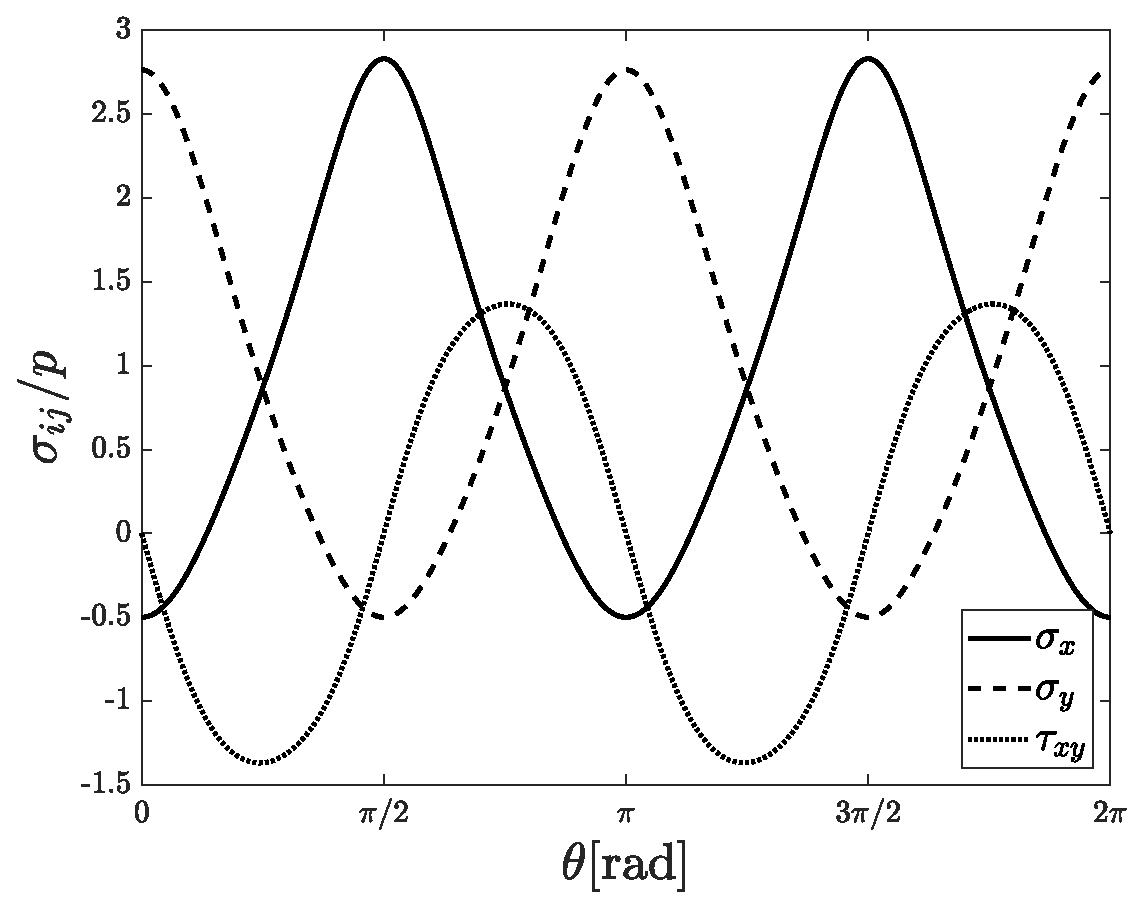
\includegraphics[width=1\linewidth, height=0.8\linewidth]{figures/stress_cartesian.eps} 
            \caption{}
            \label{fig:stress_cartesian}
        \end{subfigure}
        \begin{subfigure}{0.5\textwidth}
            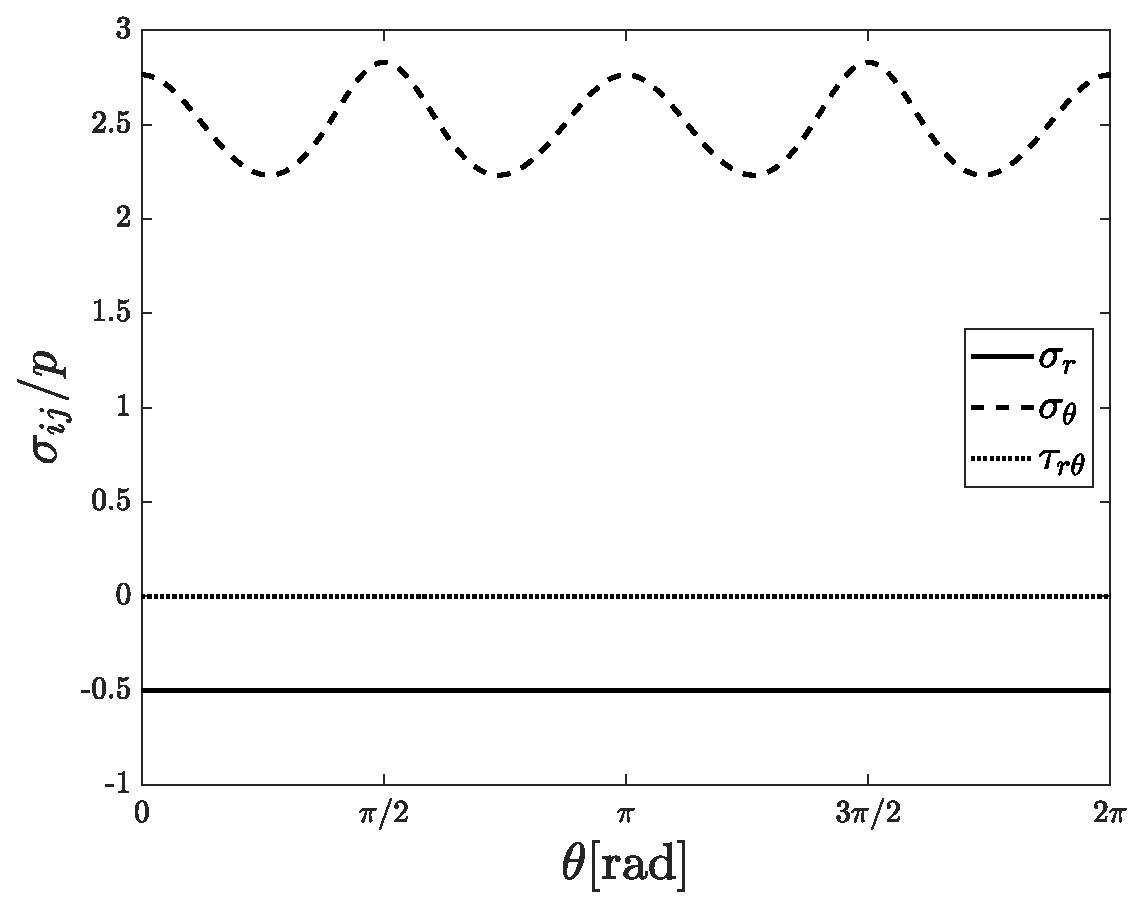
\includegraphics[width=1\linewidth, height=0.8\linewidth]{figures/stress_polar.eps} 
            \caption{}
            \label{fig:stress_polar}
        \end{subfigure}
    \caption{Normalized stress distributions on the hole edge in (a) Cartesian (b) Polar coordinate system.}
    % \label{}
\end{figure}

Despite the sinusoidal behavior of the Cartesian stress components in \cref{fig:stress_cartesian}, the polar stress provides a better insight into stress distribution on the hole edge (\cref{fig:stress_polar}). The radial stress, $\sigma_r$, and shear stress, $\tau_{r\theta}$, coincide with their prescribed traction value on the hole boundary (see \cref{fig:traction_element}). The hoop stress, $\sigma_{\theta}$, various sinusoidally on the hole edge and has the highest stress value (almost 5$\sigma_r$ on average).

\begin{figure}[ht]
    \centering
    \includegraphics[width = 0.5\textwidth ]{figures/traction_element.pdf}
    \caption{Stress components on the hole edge.}
    \label{fig:traction_element}
\end{figure}

The stress field around the hole are plotted in \cref{fig:stress_on_x} and \cref{fig:stress_on_y}. As is seen, all the stress components converge to their value at infinity. Approaching the hole edge, $\sigma_x$ and $\sigma_y$ go to infinity and $\tau_{xy}$ changes sign from $+\infty$ to $-\infty$ which does not affect our solution as they are inside the hole and do not represent any physical meaning. \\

\begin{figure}[ht]
        \begin{subfigure}{0.5\textwidth}
            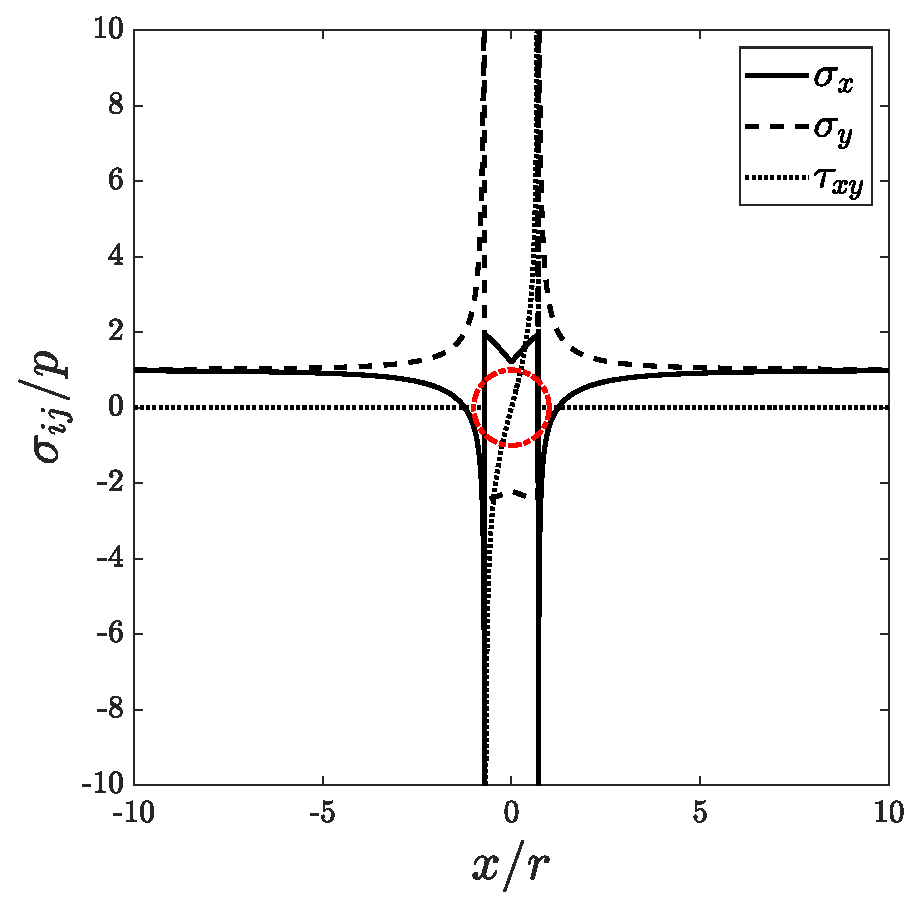
\includegraphics[width=1\linewidth]{figures/stress_on_x.eps} 
            \caption{}
            \label{fig:stress_on_x}
        \end{subfigure}
        \begin{subfigure}{0.5\textwidth}
            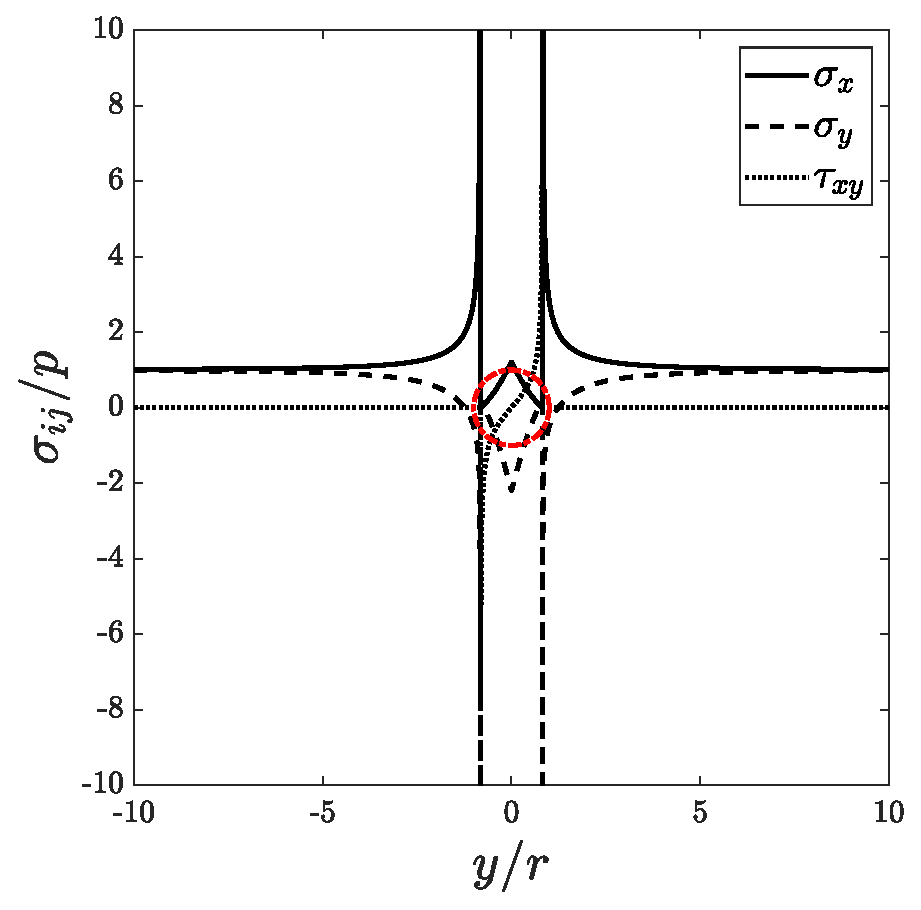
\includegraphics[width=1\linewidth]{figures/stress_on_y.eps} 
            \caption{}
            \label{fig:stress_on_y}
        \end{subfigure}
    \caption{Normalized stress distributions along (a) $x$-axis (b) $y$-axis. The circle designates the hole.}
    % \label{}
\end{figure}

In order to get an overview of which stress field plays a key role around the hole, the plot of the polar stress components at distances of 5 and 10 times the hole radius are also added and compared in \cref{fig:polar_stress_at_distance}. $\sigma_{\theta}$ is the highest on the hole edge and reduces as we move away from the hole. The absolute value of $\sigma_r$ increases by moving in the opposite direction towards the external boundary as it converges to its value at infinity. For this loading condition, $\tau_{r\theta}$ is zero everywhere as expected. \\

The deformation around the whole can be calculated from \cref{eq:u_v}. \cref{fig:deformation} shows the resultant hole deformation calculated from 

\begin{equation*}
    u_t = \sqrt{v^2 + v^2}
\end{equation*}



The deformed hole is shown in \cref{fig:deformation}. Unlike an isotropic material which deforms uniformly, the composite laminate undergoes more deformation in the $y$-axis than the $x$-axis which is due to the stacking sequence (the majority (40\%) of the layers are 0) and smaller transverse Young's modulus compared to the longitudinal. The separate plots of normalized $u$ and $v$ around the hole are also given in \cref{fig:displacement}.

\section{Conclusion}
Lekhnitskii formalism is a powerful tool in analyzing the anisotropic elastic bodies and has many applications in aerospace. In this report, we revisited Lekhnitskii theory and applied it to a thin phototropic laminate with a circular hole. During the development, we utilized the two-dimensional general stress and assumed that the external boundary condition does not influence the hole. The result show that the hole disturbs the stress field in the body inducing a high stress region in the vicinity of the hole.


\begin{figure}[H]
        \begin{subfigure}{0.5\textwidth}
            \includegraphics[width=1\linewidth, height=0.8\linewidth]{figures/sigma_r.eps} 
            \caption{}
            \label{fig:sigma_r}
        \end{subfigure}
        \begin{subfigure}{0.5\textwidth}
            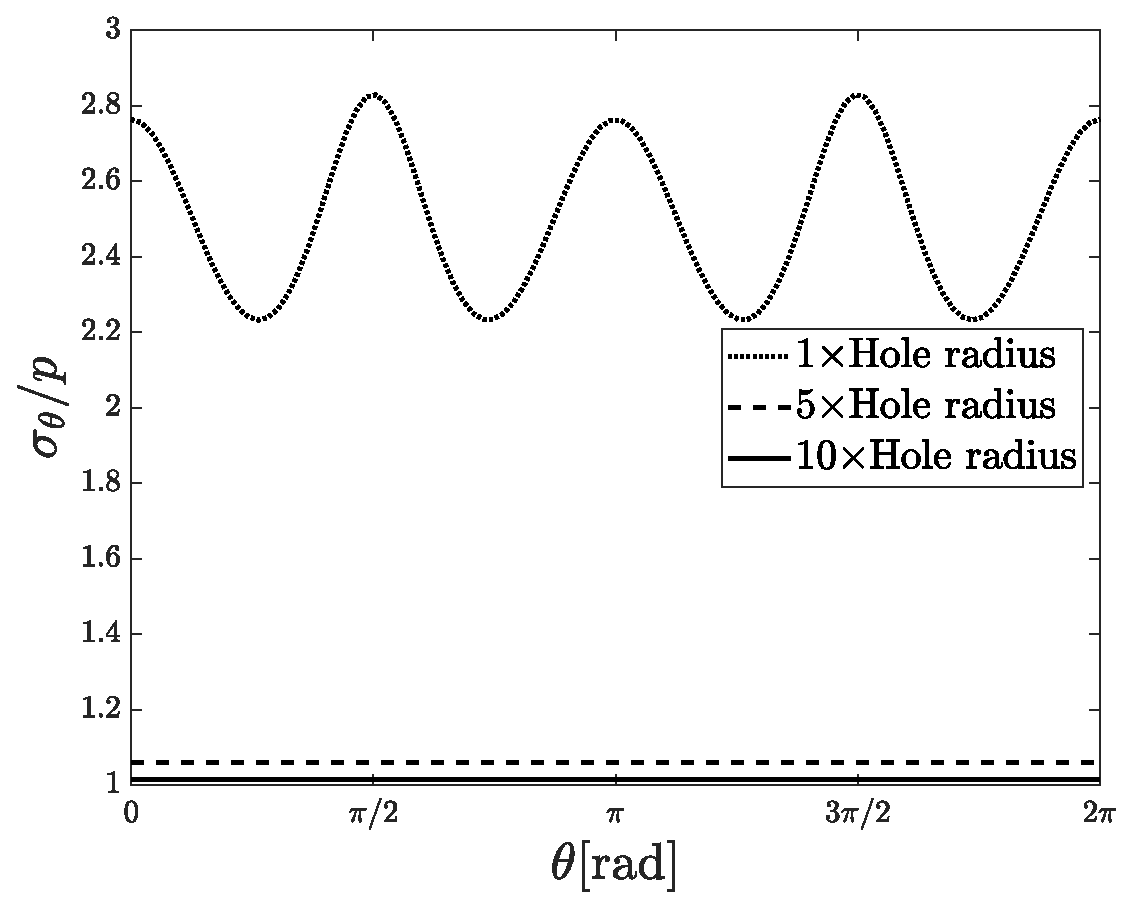
\includegraphics[width=1\linewidth, height=0.8\linewidth]{figures/sigma_theta.eps} 
            \caption{}
            \label{fig:sigma_theta}
        \end{subfigure}
        \begin{subfigure}{0.5\textwidth}
            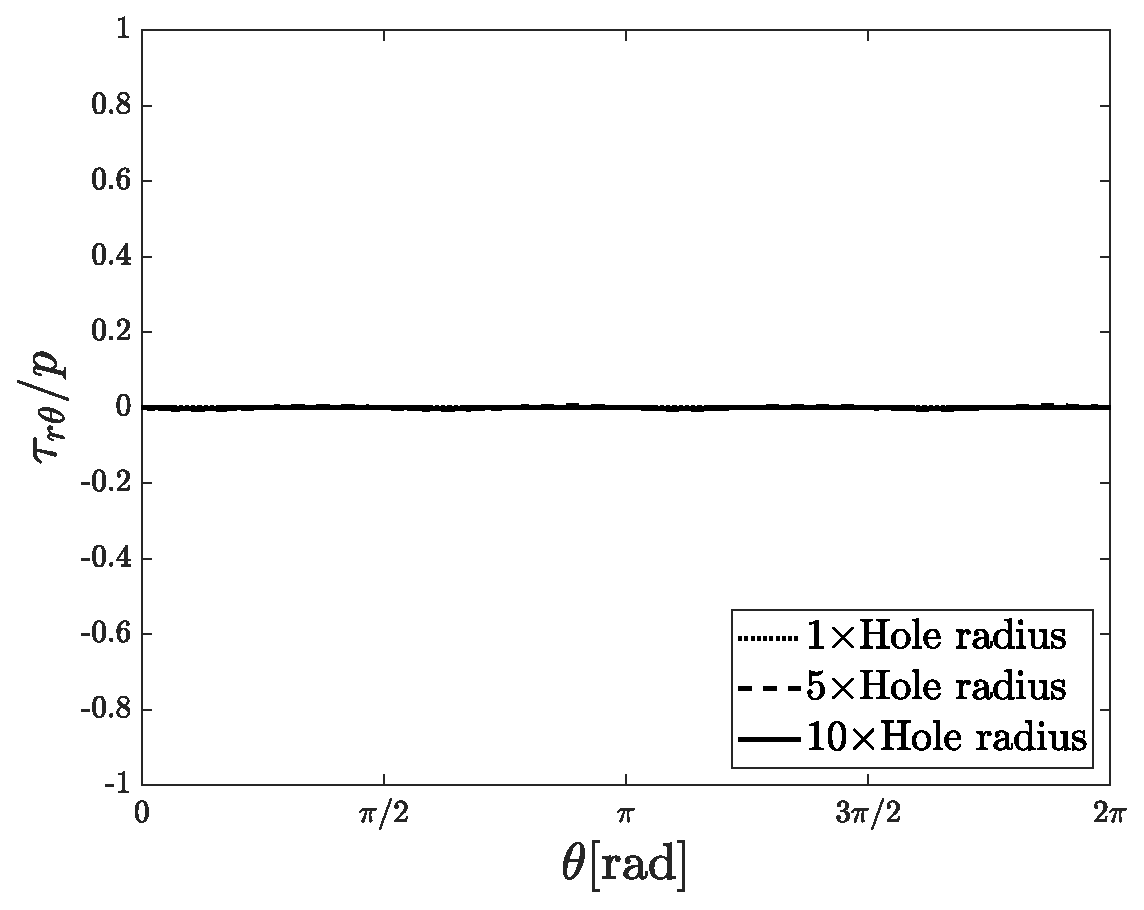
\includegraphics[width=1\linewidth, height=0.8\linewidth]{figures/tau_rt.eps} 
            \caption{}
            \label{fig:tau_rt}
        \end{subfigure}
    \caption{Normalized (a) radial (b) hoop (c) shear stress distributions at various distance from the hole edge.}
    \label{fig:polar_stress_at_distance}
\end{figure}



\begin{figure}[H]
        \begin{subfigure}{0.5\textwidth}
            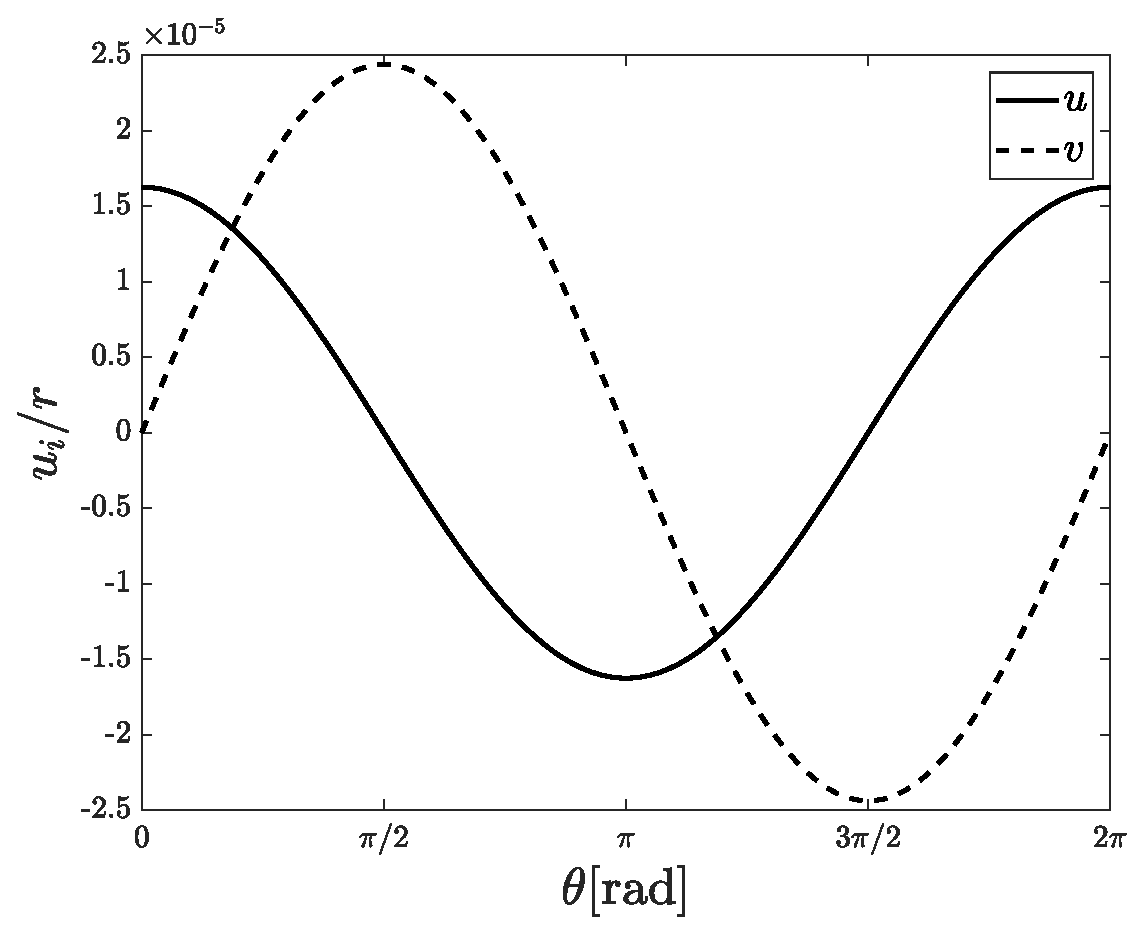
\includegraphics[width=1\linewidth]{figures/displacement.eps} 
            \caption{}
            \label{fig:displacement}
        \end{subfigure}
        \begin{subfigure}{0.5\textwidth}
            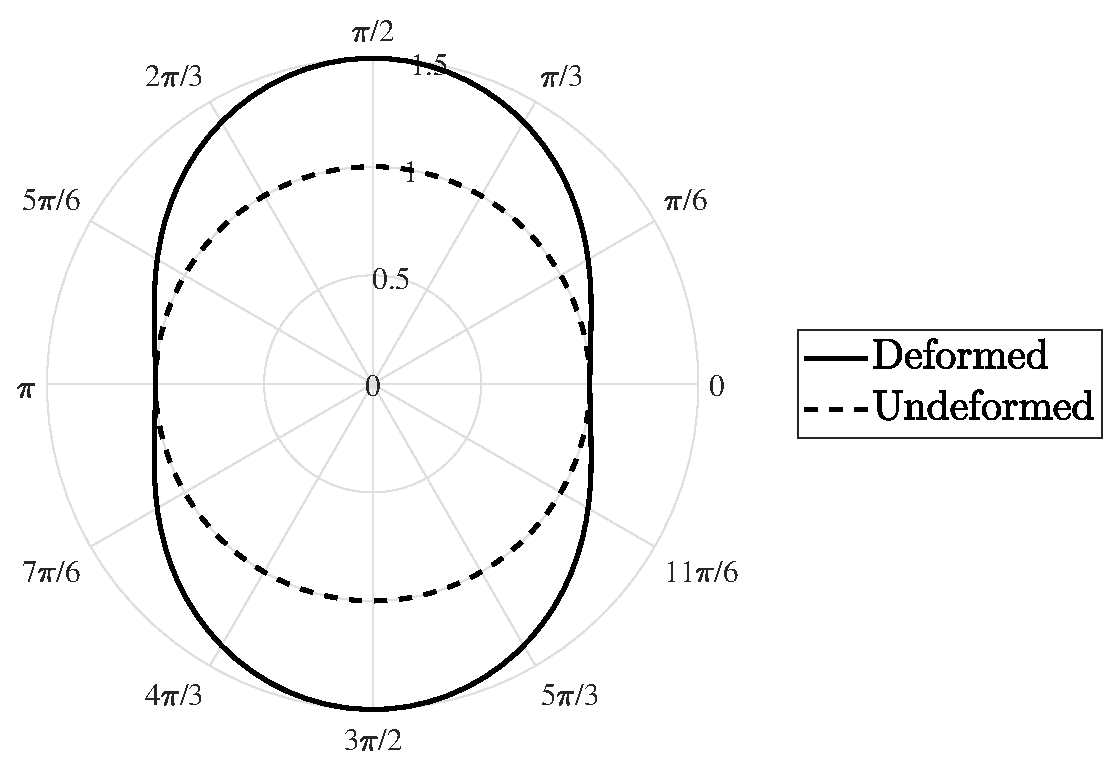
\includegraphics[width=1\linewidth]{figures/deformation.eps} 
            \caption{}
            \label{fig:deformation}
        \end{subfigure}
    \caption{(a) Normalized displacement distribution around the hole. (b) Total deformation of circular hole.}
    % \label{}
\end{figure}

\appendix
\section*{Appendices}
\section{Components of the Compliance Tensor} \label{app:compliance_mat}
The compliance tensor for a general laminate can be calculated from the tensor transformation rule. As the compliance is a fourth-order tensor, the compliance tensor in the transformed coordinate, $\bm{S^{'}}$, is

\begin{equation*}
    S^{'}_{ijkl} = Q_{pi} Q_{qj} Q_{rk} Q_{sl} S_{pqrs}
\end{equation*}

where $Q$ is the proper orthogonal tensor .The compliance tensor components become \cite{Kassapoglou2015}

\begin{flalign}
    & S^{'}_{11} = S_{11} c^4 + (2 S_{12} + S_{66}) s^2 c^2 + S_{22} s^4 & \notag \\
    & S^{'}_{12} = S_{12} (c^4 + s^4) + (S_{11} + S_{22} - S_{66}) s^2 c^2 &  \notag \\
    & S^{'}_{13} = S_{13} c^2 + S_{23} s^2 & \notag \\
    & S^{'}_{16} = (2 S_{11} - 2 S_{12} - S_{66}) s c^3 + (2 S_{12} - 2 S_{22} + S_{66}) c s^3 & \notag \\
    & S^{'}_{22} = S_{11} s^4 + S_{22} c^4 + (2 S_{12} + S_{66}) s^2 c^2 & \notag \\
    & S^{'}_{23} = S_{13} s^2 + S_{23} c^2 & \notag \\
    & S^{'}_{26} = (2 S_{12} - 2 S_{22} + S_{66}) s c^3 + (2 S_{11} - 2 S_{12} - S_{66}) c s^3 & \notag \\
    & S^{'}_{33} = S_{33} & \notag \\
    & S^{'}_{36} = 2 (S_{13} - S_{23}) s c & \notag \\
    & S^{'}_{44} = S_{44} c^2 + S_{55} s^2 & \notag \\
    & S^{'}_{45} = (S_{55} - S_{44}) s c & \notag \\
    & S^{'}_{55} = S_{44} s^2 + S_{55} c^2 & \notag \\
    & S^{'}_{66} = 4 (S_{11} - 2 S_{12} + S_{22}) c^2 s^2 + (s^2 - c^2)^2 S_{66}
    \label{eq:general_compliance}
\end{flalign}

where 

\begin{equation*}
    \begin{matrix}
    S_{11} = \dfrac{1}{E_{11}} & , 
    S_{12} = -\dfrac{\nu_{12}}{E_{11}} & , 
    S_{13} = -\dfrac{\nu_{13}}{E_{11}} & ,
    S_{22} = \dfrac{1}{E_{22}} & ,
    S_{23} = -\dfrac{\nu_{23}}{E_{22}} & ,
    S_{33} = \dfrac{1}{E_{33}} & ,
    S_{44} = \dfrac{1}{\mu_{23}} &
    \\
    S_{55} = \dfrac{1}{\mu_{13}} & ,
    S_{66} = \dfrac{1}{\mu_{12}} & ,
    c = \cos(\theta) & , 
    s = \sin(\theta)
    \end{matrix}
\end{equation*}

$E_{11}$ is the longitudinal Young's modulus, $E_{22}$ and $E_{33}$ are transverse Young's moduli, $\mu_{12}$ and $\mu_{13}$ are in-plane shear moduli, $\mu_{23}$ is the out-of-plane shear modulus, $\nu_{12}$ and $\nu_{13}$ are in-plane Poisson's ratios and $\nu_{23}$ is the out-of-plane Poisson's ratio. The compliance tensor for an orthotropic laminate is

\begin{equation}
\bm{S}
=\begin{bmatrix}
\dfrac{1}{E_{11}} & -\dfrac{\nu_{12}}{E_{11}} & -\dfrac{\nu_{13}}{E_{11}} & 0 & 0 & 0 \\ 
-\dfrac{\nu_{12}}{E_{11}} & \dfrac{1}{E_{22}} & -\dfrac{\nu_{23}}{E_{22}} & 0 & 0 & 0 \\ 
-\dfrac{\nu_{13}}{E_{11}} & -\dfrac{\nu_{23}}{E_{22}} & \dfrac{1}{E_{33}} & 0 & 0 & 0 \\ 
0 & 0 & 0 & \dfrac{1}{\mu_{23}} & 0 & 0 \\ 
0 & 0 & 0 & 0 & \dfrac{1}{\mu_{31}} & 0 \\ 
0 & 0 & 0& 0 & 0 & \dfrac{1}{\mu_{12}}
\end{bmatrix}
\label{eq:ortho_compliance}
\end{equation}

\section{Derivation of the Compatibility Equation} \label{app:compatibility_eqn}

The strain-displacement relation is

\begin{equation*}
    \begin{matrix}
    \epsilon_x = \dfrac{\partial u}{\partial x} & , 
    \epsilon_y = \dfrac{\partial v}{\partial y} & , 
    \gamma_{xy} = \dfrac{\partial u}{\partial y} + \dfrac{\partial v}{\partial x}
    \end{matrix}
\end{equation*}

Differentiating $\epsilon_x$ and $\epsilon_y$ w.r.t $y$ and $x$ twice together with differentiating $\gamma_{xy}$ w.r.t $x$ and then $y$ give

\begin{equation*}
    \begin{matrix}
    \dfrac{\partial^2 \epsilon_x}{\partial y^2} = \dfrac{\partial^3 u}{\partial y^2 \partial x} & , 
    \dfrac{\partial^2 \epsilon_y}{\partial x^2} = \dfrac{\partial^3 v}{\partial x^2 \partial y} & ,
    \dfrac{\partial^2 \gamma_{xy}}{\partial x \partial y} = \dfrac{\partial^3 u}{\partial x \partial y^2} + \dfrac{\partial^3 v}{\partial x^2 \partial y}
    \end{matrix}
\end{equation*}

Summing the first two terms and then subtracting the third term yield the compatibility equation.

\begin{equation*}
    \dfrac{\partial^2 \epsilon_x}{\partial y^2} + \dfrac{\partial^2 \epsilon_y}{\partial x^2} - \dfrac{\partial^2 \gamma_{xy}}{\partial x \partial y} = 0
\end{equation*}
\section{Derivation of Compatibility Equation in Terms of Stress Function for the Plane Deformation Case} \label{app:plane_strain}

Let us assume

\begin{equation*}
    \begin{matrix}
    u = u(x, y) & , 
    v = v (x, y) & , 
    w = 0
    \end{matrix}
\end{equation*}

thus we have

\begin{equation*}
    \begin{matrix}
    \epsilon_x = \dfrac{\partial u}{\partial x} & , 
    \epsilon_y = \dfrac{\partial v}{\partial y} & , 
    \gamma_{xy} = \dfrac{\partial u}{\partial y} + \dfrac{\partial v}{\partial x} & , 
    \epsilon_z = \gamma_{yz} = \gamma_{zx} = 0
    \end{matrix}
\end{equation*}

The stress and strain can be correlated using the inverse of the compliance matrix in \cref{eq:stress_strain} or the so-called reduced transformation matrix, $\bm{Q}$.

\begin{equation}
\begin{Bmatrix}
\overline{\epsilon}_x\\ 
\overline{\epsilon}_y\\ 
0\\ 
\overline{\gamma}_{xy}\\
\end{Bmatrix}
=\begin{bmatrix}
Q_{11} & Q_{12} & Q_{13} & Q_{16} \\ 
Q_{12} & Q_{22} & Q_{23} & Q_{26} \\ 
Q_{13} & Q_{23} & Q_{33} & Q_{36} \\ 
Q_{16} & Q_{26} & Q_{36} & Q_{66} 
\end{bmatrix}
\begin{Bmatrix}
\overline{\sigma}_x\\ 
\overline{\sigma}_y\\ 
\overline{\sigma}_z\\ 
\overline{\tau}_{xy}\\
\end{Bmatrix}
\label{eq:stress_strain_reduced}
\end{equation}

where \cite{Lekhnitskii1968}

\begin{equation*}
    Q_{ij} = S_{ij} - \dfrac{S_{i3} S_{j3}}{S_{33}} \quad\quad (i, j = 1, 2, 6)
\end{equation*}

$\overline{\sigma}_z$ can be solved from \cref{eq:stress_strain_reduced}.

\begin{equation*}
    \sigma_z = -\dfrac{Q_{13} \sigma_x + Q_{23} \sigma_y + Q_{36} \tau_{xy}}{Q_{33}}
\end{equation*}

Invoking \cref{eq:average_stress} and \cref{eq:stress_strain_reduced}, we get an analogous equation to \cref{eq:pde_body_included} with different constants.

\begin{multline*}
    Q_{22} \frac{\partial^4 \phi}{\partial x^4} - 2 Q_{26} \frac{\partial^4 \phi}{\partial x^3 \partial y} + (2 Q_{12} + Q_{66}) \frac{\partial^4 \phi}{\partial x^2 \partial y^2} - 2 Q_{16} \frac{\partial^4 \phi}{\partial x \partial y^3} + Q_{11} \frac{\partial^4 \phi}{\partial y^4} \\ + (Q_{12} + Q_{22}) \frac{\partial^2 \overline{V}}{\partial x^2} - (Q_{16} + Q_{26}) \frac{\partial^2 \overline{V}}{\partial x \partial y}  + (Q_{11} + Q_{12}) \frac{\partial^2 \overline{V}}{\partial y^2} = 0
\end{multline*}

which reduces to below, in case of zero body forces.

\begin{equation*}
    Q_{22} \frac{\partial^4 \phi}{\partial x^4} - 2 Q_{26} \frac{\partial^4 \phi}{\partial x^3 \partial y} + (2 Q_{12} + Q_{66}) \frac{\partial^4 \phi}{\partial x^2 \partial y^2} - 2 Q_{16} \frac{\partial^4 \phi}{\partial x \partial y^3} + Q_{11} \frac{\partial^4 \phi}{\partial y^4} = 0
\end{equation*}

See \texttt{pde$\_$plane$\_$strain.mw} for the corresponding Maple file. 
\section{Proof of \texorpdfstring{$\phi(x, y) = f(z)$}{}}\label{app:why_z_is_complex}
The proof of this section is provided in \cite{Koussios2015}. The compatibility equation in terms of potential stress function reduces to below based on the assumptions in \cref{sec:solve_pde}.

\begin{equation*}
    r^2 \frac{\partial^4 \phi(x, y)}{\partial x^4} + 2a \frac{\partial^4 \phi(x, y)}{\partial x^2 \partial y^2} + \frac{\partial^4 \phi(x, y)}{\partial y^4} = 0
\end{equation*}

Using the "," operator instead of partial differentiation, the above equation becomes

\begin{equation*}
    r^2 \phi(x, y)_{,xxxx} + 2a \phi(x, y)_{,xxyy} + \phi(x, y)_{,yyyy} = 0
\end{equation*}

Replace $r^2$ and $2a$ with $\xi^2\lambda^2$ and $-(\xi^2 + \lambda^2)$, where both $\xi$ and $\lambda$ are independent constants.

\begin{gather*}
    \xi^2\lambda^2 \phi(x, y)_{,xxxx} -(\xi^2 + \lambda^2) \phi(x, y)_{,xxyy} + \phi(x, y)_{,yyyy} = 0 \notag\\
    (\xi^2 \phi(x, y)_{,xx} - \phi(x, y)_{,yy})(\lambda^2 \phi(x, y)_{,xx} - \phi(x, y)_{,yy}) = 0 \notag\\
    (\xi \phi(x, y)_{,x} + \phi(x, y)_{,y}) (\xi \phi(x, y)_{,x} - \phi(x, y)_{,y}) (\lambda \phi(x, y)_{,x} + \phi(x, y)_{,y}) (\lambda \phi(x, y)_{,x} - \phi(x, y)_{,y}) = 0
\end{gather*}

As a result, each term in the last line of the above set of equations should be zero. Let us continue with $\xi \phi(x, y)_{,x} - \phi(x, y)_{,y}$. The same strategy is applicable to the rest of the terms. 

\begin{gather*}
    \xi \phi(x, y)_{,x} - \phi(x, y)_{,y} = 0\notag\\
    \{ \phi(x, y)_{,x} \quad \phi(x, y)_{,y}\} 
    \begin{Bmatrix}
    \xi\\ 
    -1
    \end{Bmatrix} = 0
\end{gather*}

for the above equation to be valid, 

\begin{equation*}
    \begin{Bmatrix}
    \phi(x, y)_{,x}\\ 
    \phi(x, y)_{,y}
    \end{Bmatrix} = 
    \begin{Bmatrix}
    1\\ 
    \xi
    \end{Bmatrix}
\end{equation*}

The function that satisfies the above is $\phi(x, y) = f(x + \xi y)$ which is a complex function.




\section{Determination of the Characteristic Equation Roots}\label{app:complex_imag_roots}
For an ideal elastic body $r+a$ is always positive.

\begin{gather*}
    r = \sqrt{\dfrac{S_{22}}{S_{11}}} = \sqrt{\dfrac{E_{11}}{E_{22}}} > 0
\end{gather*}

For an ideal elastic laminate, $0<\nu_{12}<\dfrac{1}{2}$.

\begin{gather*}
    2a = \dfrac{2S_{12} + S_{66}}{S_{11}} = \dfrac{-2\dfrac{\nu_{12}}{E_{11}} + \dfrac{1}{\mu_{12}}}{\dfrac{1}{E_{11}}} = \dfrac{E_{11} - 2 \mu_{12} \nu_{12}}{\mu_{12}} \xrightarrow[]{E_{11}>\mu_{12}>0} \dfrac{E_{11} - 2 \mu_{12} \nu_{12}}{\mu_{12}} > 0
\end{gather*}

Next, for 

\subsubsection*{Case 1: \texorpdfstring{$r - a\geq 0$}{}}

\begin{gather}
    s_1 = \sqrt{\dfrac{r-a}{2}} + i \sqrt{\dfrac{r+a}{2}} \notag\\
    s_2 = -\sqrt{\dfrac{r-a}{2}} + i \sqrt{\dfrac{r+a}{2}} \notag\\
    s_3 = \sqrt{\dfrac{r-a}{2}} - i \sqrt{\dfrac{r+a}{2}} \notag\\
    s_4 = -\sqrt{\dfrac{r-a}{2}} - i \sqrt{\dfrac{r+a}{2}}
    \label{eq:s1_s4_complex}
\end{gather}

then, $s_1$ to $s_4$ are all complex.

\subsubsection*{Case 2: \texorpdfstring{$r - a < 0$}{}}

\begin{gather}
    s_1 = i \left( \sqrt{\dfrac{a-r}{2}} + \sqrt{\dfrac{r+a}{2}} \right) \notag\\
    s_2 = i \left( -\sqrt{\dfrac{a-r}{2}} + \sqrt{\dfrac{r+a}{2}} \right) \notag\\
    s_3 = -i \left( -\sqrt{\dfrac{a-r}{2}} + \sqrt{\dfrac{r+a}{2}} \right) \notag\\
    s_4 = -i \left( \sqrt{\dfrac{a-r}{2}} + \sqrt{\dfrac{r+a}{2}} \right)
    \label{eq:s1_s4_imaginary}
\end{gather}

then, $s_1$ to $s_4$ are all imaginary.
\section{Derivation of Traction Equation on the Internal Boundary Due to An Opening}\label{app:internal}

\begin{equation*}
\left\{\begin{matrix}
    \left(\dfrac{\partial^2 \phi}{\partial y^2} + V \right) \dfrac{-\mathrm{d}y}{\mathrm{d}s} - \dfrac{\partial^2 \phi}{\partial x \partial y}  \dfrac{\mathrm{d}x}{\mathrm{d}s} = X   \\
    \\
    \dfrac{\partial^2 \phi}{\partial x \partial y}  \dfrac{\mathrm{d}y}{\mathrm{d}s} + \left( \dfrac{\partial^2 \phi}{\partial x^2} + V \right) \dfrac{-\mathrm{d}x}{\mathrm{d}s} = Y  
\end{matrix}\right.
\end{equation*}
%%%%%%%%%%%%%%%%%%%%
\begin{equation*}
\left\{\begin{matrix}
    \dfrac{\partial^2 \phi}{\partial y^2} \dfrac{\mathrm{d}y}{\mathrm{d}s} + \dfrac{\partial^2 \phi}{\partial x \partial y}  \dfrac{\mathrm{d}x}{\mathrm{d}s} = -X - V \dfrac{\mathrm{d}y}{\mathrm{d}s} \\
    \\
    \dfrac{\partial^2 \phi}{\partial x \partial y}  \dfrac{\mathrm{d}y}{\mathrm{d}s} + \dfrac{\partial^2 \phi}{\partial x^2} \dfrac{\mathrm{d}x}{\mathrm{d}s} = Y - V \dfrac{\mathrm{d}x}{\mathrm{d}s}  
\end{matrix}\right.
\end{equation*}
%%%%%%%%%%%%%%%%%%%%
\begin{equation*}
\left\{\begin{matrix}
    \dfrac{\partial}{\partial y}\left( \dfrac{\partial \phi}{\partial y} \right) \dfrac{\mathrm{d}y}{\mathrm{d}s} + \dfrac{\partial}{\partial x}\left( \dfrac{\partial \phi}{\partial y} \right) \dfrac{\mathrm{d}x}{\mathrm{d}s} = -X - V \dfrac{\mathrm{d}y}{\mathrm{d}s}\\
    \\
    \dfrac{\partial}{\partial y}\left( \dfrac{\partial \phi}{\partial x} \right) \dfrac{\mathrm{d}y}{\mathrm{d}s} + \dfrac{\partial}{\partial x}\left( \dfrac{\partial \phi}{\partial x} \right) \dfrac{\mathrm{d}x}{\mathrm{d}s} = Y - V \dfrac{\mathrm{d}x}{\mathrm{d}s}  
\end{matrix}\right.
\end{equation*}

From \cref{eq:ds}

\begin{equation*}
\left\{\begin{matrix}
    \dfrac{\partial}{\partial s}\left( \dfrac{\partial \phi}{\partial y} \right) = -X - V \dfrac{\mathrm{d}y}{\mathrm{d}s}\\
    \\
    \dfrac{\partial}{\partial y}\left( \dfrac{\partial \phi}{\partial x} \right) = Y - V \dfrac{\mathrm{d}x}{\mathrm{d}s}  
\end{matrix}\right.
\end{equation*}
%%%%%%%%%%%%%%%%%%%%
\begin{equation*}
\left\{\begin{matrix}
    \dfrac{\partial \phi}{\partial y} = \displaystyle\int_{s_0}^{s_1}{\left (-X - V \dfrac{\mathrm{d}y}{\mathrm{d}s}\right)} \mathrm{d}s + c_3\\
    \\
    \dfrac{\partial \phi}{\partial x} = \displaystyle\int_{s_0}^{s_1}{\left(Y - V \dfrac{\mathrm{d}x}{\mathrm{d}s}\right)}\mathrm{d}s + c_4\\ 
\end{matrix}\right.
\end{equation*}
\section{On the Selection of Hole Radius}\label{app:why_r_is_one}
Take the general case of an ellipse in polar coordinate system where

\begin{equation*}
    \begin{matrix}
    x = d \cos\theta & , 
    y = b \sin\theta
    \end{matrix}
\end{equation*}

$z$ in its complex form can be written as 

\begin{align*}
    z & =  x + iy = d \cos\theta + i b \sin\theta \overset{(1)}{=} d \cos\theta - i d \sin\theta + i b \sin\theta + i d \sin\theta \overset{(2)}{=} d e^{i\theta} + i(b-d)\sin\theta & \\
    & \overset{(3)}{=} d e^{i\theta} + \left( \dfrac{b -d}{2} \right) (e^{i\theta} - e^{-i\theta}) = \left(\dfrac{b+d}{2} \right) e^{i\theta} - \left( \dfrac{b-d}{2} \right) e^{-i\theta}
\end{align*}

where we 

\begin{align*}
    \begin{matrix}
    \text{added and subtract} & i d \sin\theta \quad & \text{in (1)}
    \end{matrix} \\
    \begin{matrix}
    \text{utilized Euler's formula} & e^{-i\theta} = \cos \theta - i \sin \theta \quad & \text{in (2)}
    \end{matrix} \\
\end{align*}

\begin{align*}
    \begin{matrix}
    \text{replaced} & \sin\theta = \dfrac{e^{i\theta} - e^{-i\theta}}{2} \quad & \text{in (3)}
    \end{matrix}
\end{align*}

Based on the above equation \cite{Jong1987}

\begin{align*}
    z_k = & \left(\dfrac{d - i s_k b}{2} \right) e^{i\theta} + \left( \dfrac{d + i s_k b}{2} \right) e^{-i\theta} & \\
    \overset{z = e^{i\theta}}{=} & \left(\dfrac{d - i s_k b}{2} \right) z + \left( \dfrac{d + i s_k b}{2} \right) \dfrac{1}{z} & \\
    \Rightarrow & (d - i s_k b) z^2  - 2 z_k z + (d + i s_k b)= 0
\end{align*}

Solving for the roots, $\zeta_k$, of the above equation (we use $\zeta_k$ instead of $z_k$ to avoid possible misinterpretation caused by $z_k$ in \cref{eq:phi_in_form_f} to \cref{eq:final_sol})

\begin{equation}
    \begin{matrix}
    \zeta_k = \dfrac{2 z_k \pm \sqrt{4 z_k^2 - 4(d + i s_k b) (d - i s_k b)}}{d - i s_k b} = \dfrac{z_k \pm \sqrt{z_k^2 - s_k^2 b^2 - d^2}}{d - i s_k b} &
    \text{where} \quad k = 1, 2
    \end{matrix}
    \label{eq:zeta_k_ellipse}
\end{equation}

For a circular opening ($d=b=1$) with a radius $r$, to be on the edge, $|z|=r$, and

\begin{equation}
    \zeta_k = \dfrac{z_k/r \pm \sqrt{(z_k/r)^2 - s_k^2 - 1}}{1 - i s_k}
    \label{eq:zeta_k_circle}
\end{equation}

The unitless parameter $z_k/r$, on the circle, can be replaced with unity; hence, $z_k/r$ can be simply written as $z_k$ and the hole radius can be assumed as one.


\section{Derivation of \texorpdfstring{$A_k$}{} constants for A Harmonic Load on the Hole Edge} \label{app:remove_A_k}

For the general case of harmonic load, \cref{eq:harmonic_load}, we replace $X$ and $Y$ in \cref{eq:A_k_1} by \cref{eq:decompose_N_T}.

\begin{gather*}
    2 \mathfrak{Re}[s_1 A_1 \ln z_1 + s_2 A_2 \ln z_2]  \begin{matrix} s_1 \\ s_0 \end{matrix} = 
-\displaystyle\int_{s_0}^{s_1}{N(m, \theta) \cos\theta - T(m, \theta) \sin\theta} \mathrm{d}s \\
    2 \mathfrak{Re}[A_1 \ln z_1 + A_2 \ln z_2]     \begin{matrix}  s_1 \\ s_0 \end{matrix}
= \displaystyle\int_{s_0}^{s_1}{N(m, \theta) \cos\theta + T(m, \theta) \sin\theta}\mathrm{d}s
\end{gather*}

Integrating on the hole ($0 \leq \theta \leq 2\pi$)

\begin{gather*}
    s_1 A_1 + s_2 A_2 - \overline{s_1} \overline{A_1} - \overline{s_2} \overline{A_2} = -\displaystyle\int_{0}^{2\pi}{N(m, \theta) \cos\theta - T(m, \theta) \sin\theta} \mathrm{d}\theta = 0 \\
    A_1 + A_2 - \overline{A_1} - \overline{A_2} = \displaystyle\int_{0}^{2\pi}{N(m, \theta) \cos\theta + T(m, \theta) \sin\theta}\mathrm{d}\theta = 0
\end{gather*}

Due to the absence of the resultant load, $R_x = R_y = 0$ on the hole edge, as is the case for the harmonic traction, then $A_1 = A_2 = \overline{A_1} = \overline{A_2} = 0$; thus, $\displaystyle\sum_{k=1}^{2}{A_k \ln z_k}$ vanishes.
\section{Mapping \texorpdfstring{$g_n^{(k)} z_k^{-n}$}{} to \texorpdfstring{$c_n^{(k)} \zeta_k^{-n}$}{}} \label{app:mapping}

For a circular hole ($r=1$),

\begin{equation*}
    \begin{matrix}
    x = \cos\theta & , 
    y = \sin\theta
    \end{matrix}
\end{equation*}

\begin{align*}
    \zeta_k & = \dfrac{z_k \pm \sqrt{z_k^2 - s_k^2 - 1}}{1-is_k} = \dfrac{x + s_k y \pm \sqrt{(x + s_k y)^2 - s_k^2 - 1}}{1-is_k} & \\
    &= \dfrac{\cos\theta + s_k \sin\theta \pm \sqrt{(\cos\theta + s_k \sin\theta)^2 - s_k^2 -1}}{1 - i s_k} & \\
    & = \dfrac{\cos\theta + s_k \sin\theta \pm \sqrt{\cos^2\theta + s_k^2 \sin^2\theta + 2s_k\cos\theta \sin\theta - s_k^2 -1}}{1 - i s_k}  & \\
    & = \dfrac{\cos\theta + s_k \sin\theta \pm \sqrt{-(1 - \cos^2\theta) - s_k^2 (1- \sin^2\theta) + 2s_k\cos\theta \sin\theta}}{1 - i s_k}  & \\
    & = \dfrac{\cos\theta + s_k \sin\theta \pm \sqrt{-\sin^2\theta - s_k^2 \cos^2\theta + 2s_k\cos\theta \sin\theta}}{1 - i s_k}  & \\
    & = \dfrac{\cos\theta + s_k \sin\theta \pm \sqrt{(\sin^2\theta - s_k^2 \cos^2\theta)^2}}{1 - i s_k}  & \\
    & = \dfrac{\cos\theta + s_k \sin\theta \pm i(\sin\theta - s_k \cos\theta)}{1 - i s_k}  & \\
\end{align*}

Let us replace $\pm$ with $\mathfrak{S}$ as it is required to determine the proper sign during the solution. The sign selection is given in Algorithm \ref{alg:sign_selection}.

\begin{align*}
    \zeta_k & = \dfrac{\cos\theta + s_k \sin\theta + \mathfrak{S} i(\sin\theta - s_k \cos\theta)}{1 - i s_k} \overset{\mathfrak{S}=1}{=} \dfrac{\cos\theta(1-i s_k) + \sin\theta (s_k+i)}{1 - i s_k} & \\
    & = \dfrac{\cos\theta(1-i s_k) + i \sin\theta (1 - i s_k)}{1 - i s_k} = \cos\theta + i\sin\theta = e^{i\theta} = z  &
\end{align*}

which is true when we are on the hole edge. In fact, on the hole edge $\zeta_1 = \zeta_2 = z$.

\newpage
\bibliography{ref}
\bibliographystyle{ieeetr}

\end{document}